
\documentclass[smallextended]{svjour3}
 
\usepackage[authoryear,square]{natbib} 

%no bookmarks - conf' requirements.
\usepackage[bookmarks=false]{hyperref}
\pdfminorversion=5

\usepackage{array}
\usepackage{booktabs}
\usepackage{adjustbox}
\usepackage{pdfpages}

%\usepackage{cite}

\usepackage[T1]{fontenc}
\usepackage[utf8]{inputenc}
\include{pslatex}

\usepackage{floatrow}
\usepackage{fancyvrb}
\usepackage[flushleft]{threeparttable}

\usepackage{framed}
\makeatletter
\renewenvironment{framed}{%
 \def\FrameCommand##1{\hskip\@totalleftmargin
 \fboxsep=\FrameSep\fbox{##1}
     \hskip-\linewidth \hskip-\@totalleftmargin \hskip\columnwidth}%
 \MakeFramed {\advance\hsize-\width
   \@totalleftmargin\z@ \linewidth\hsize
   \@setminipage}}%
 {\par\unskip\endMakeFramed}
\makeatother


% *** CODE LISTING ***
\usepackage{listings}
\usepackage{color} 
\usepackage{textcomp}
\usepackage{float}
\floatstyle{plaintop}
\newfloat{Code}{H}{myc}
\definecolor{lbcolor}{rgb}{0.95,0.95,0.95} 

\usepackage{graphicx} 

\lstset{
	language=sh,
	keywordstyle=\bfseries\ttfamily\color[rgb]{0,0,1},
	identifierstyle=\ttfamily,
	commentstyle=\color[rgb]{0,0,1},
	stringstyle=\ttfamily\color[rgb]{0,0,1},
	showstringspaces=false,
	basicstyle=\scriptsize\ttfamily,
	numberstyle=\tiny,
	numbers=left,
	stepnumber=1,
	numbersep=5pt,
	tabsize=2,
	breaklines=true,
	prebreak = \raisebox{0ex}[0ex][0ex]{\ensuremath{\hookleftarrow}},
	frame=tb,
	breakatwhitespace=false,
	aboveskip={\baselineskip},
	belowskip={\baselineskip},
	columns=fixed,
	upquote=true,
	extendedchars=true,
	xleftmargin=2em,
	backgroundcolor=\color[rgb]{1,1,1},
	captionpos=b,  
}

\definecolor{add_green}{rgb}{0,0.6,0}

\lstdefinelanguage{diff}{
  %morecomment=[f][\color{blue}]{@@},     % group identifier
  morecomment=[f][\color{red}]-,         % deleted lines 
  morecomment=[f][\color{add_green}]+,       % added lines (dark green)
  morecomment=[f][\color{magenta}]{---}, % Diff header lines (must appear after +,-)
  morecomment=[f][\color{magenta}]{+++},
}

\newcommand*\rot{\rotatebox{90}}

\lstnewenvironment{code}[1][]%
{
   \noindent
   \minipage{\linewidth} 
   \vspace{0.5\baselineskip}
   \lstset{basicstyle=\ttfamily\footnotesize,frame=single,#1}}
{\endminipage}


% *** MATH PACKAGES ***
%
\usepackage{amsmath}


\usepackage[utf8]{inputenc}
\usepackage{subfigure}
\usepackage{framed}

\usepackage{xspace}
\newcommand*{\eg}{e.g.,\@\xspace}
\newcommand*{\ie}{i.e.,\@\xspace}
\newcommand{\secref}[1]{Section~\ref{#1}\xspace}
\newcommand{\figref}[1]{Figure~\ref{#1}\xspace}
\newcommand{\tabref}[1]{Table~\ref{#1}\xspace}
\newcommand{\listingref}[1]{Listing~\ref{#1}\xspace}

\usepackage{relsize}
\renewcommand*{\UrlFont}{\ttfamily\smaller\relax}
\usepackage{newunicodechar}
%for awkward characters: 
\DeclareUnicodeCharacter{00A0}{~}

\hyphenation{chan-ges}

\begin{document}

\title{FEVER: An Approach to Analyze Feature-Oriented Changes and Artefact Co-Evolution in Highly Configurable Systems}
\titlerunning{FEVER: Feature Evolution and Artefact Co-evolution}

\author{Nicolas Dintzner \and Arie van Deursen \and Martin Pinzger}

\institute{Nicolas Dintzner \and Arie van Deursen
\at Software Engineering Research Group,
Delft University of Technology,
Delft, Netherlands,\\
\email{N.J.R.Dintzner@tudelft.nl},
\email{Arie.vanDeursen@tudelft.nl}
\and
Martin Pinzger
\at Software Engineering Research Group,
University of Klagenfurt,
Klagenfurt, Austria,\\
\email{martin.pinzger@aau.at}
}

\maketitle

\begin{abstract}
The evolution of highly configurable systems is known to be a challenging task. Thorough understanding of configuration options
their relationships, and their implementation in various types of artefacts (variability model, mapping, and implementation) is required
to avoid compilation errors, invalid products, or dead code.

	Recent studies focusing on co-evolution of artefacts detailed feature-oriented change scenarios, describing how
related artefacts might change over time. However, relying on manual analysis of commits, such work
do not provide the means to obtain quantitative information on the frequency of described scenarios nor
information on the exhaustiveness of the presented scenarios for the evolution of a large scale system.

	In this work, we propose FEVER and its instantiation for the Linux kernel. 
FEVER extracts detailed information on changes in variability models (KConfig files), assets (preprocessor based C code), and mappings (Makefiles).
We apply this methodology to the Linux kernel and build a dataset comprised of 15 releases of the kernel history.

	We performed an evaluation of the FEVER approach by manually inspecting the data and compared it
with commits in the system's history. The evaluation shows that FEVER accurately captures feature related changes
for more than 85\% of the 810 manually inspected commits.
We use the collected data to reflect on occurrences of co-evolution in practice. 
Our analysis shows that complex co-evolution scenarios occur in every studied release but are not among
the most frequent change scenarios, as they only occur for 8 to 13\% of the evolving features.
Moreover, only a minority of developers working on a given release 
will make changes to all artefacts related to a feature (between 10\% and 13\% of authors).

	While our conclusions are derived from observations on the evolution of the Linux kernel, we believe that they may have
implications for tool developers as well as guide further research in the field of co-evolution of artefacts.
\end{abstract}

\keywords{highly variable systems, co-evolution, feature, variability}
\begin{acknowledgements}
This publication was supported by the Dutch national program COMMIT and carried out as part of the Allegio project 
under the responsibility of the Embedded Systems Innovation group of TNO.
\end{acknowledgements}



%intro

\section{Introduction}
\label{sec:Introduction}
%Highly configurable software and its goals
\textit{Highly configurable software systems} allow end-users to tailor a system to suit their needs and expected operational context.
This is achieved through the development of \textit{configurable} components, allowing systematic reuse and mass-customization \citep{van_gurp_notion_2001}.
The benefits of such development strategies are to reduce the time to market, as mass-customization facilitates the creation of tailored solutions, and improved software quality, as re-used components are tested in various contexts \citep{clements_software_2002}.
Examples of such systems can be found in various domains, such as database management \citep{rosenmuller_fame-dbms:_2008,batory_genesis:_1988}, SOA based systems \citep{kumara_sharing_2013}, 
operating systems \citep{berger_variability_2010}, and a number\footnote{http://splc.net/fame.html}  of industrial
and open source software projects \citep{liebig_analysis_2010} among which the Linux kernel may be the best known.

% architecture of such system - specific characteristics
A constraint of such a development strategy is the  fragmentation of concerns among development artefacts in such a 
way that re-use and customization can be achieved.  
Configuration options, or \textit{features}, play a significant role in a number of inter-related artefacts of different nature.
For systems where variability is mostly resolved at build-time, features will play a role in, at least, the following three spaces \citep{neves_safe_2015,dietrich_understanding_2012}:  
\begin{enumerate}
\item \textit{the variability space} - describing available features and their allowed combinations; 
\item the \textit{implementation space}, comprised of re-usable assets, among which configurable implementation artefacts;
and finally
\item the \textit{mapping space} - relating features to assets and often supported by a build system like Makefiles;  
\end{enumerate}
%Evolution challenges
When such systems evolve, information about feature implementation across those three spaces is actively sought by engineers \citep{heider_case_2012}.
Consistent co-evolution of artefacts is a necessity adding complexity to an already non-trivial evolutionary process \citep{mens_challenges_2005}, 
occurring in both industrial \citep{hellebrand_coevolution_2014} and open-source contexts \citep{passos_coevolution_2015,hunsen_preprocessor-based_2015}.
Inconsistent modifications across the three spaces (variability, mapping, and implementation) may lead 
to the incapacity to derive products, code compilation errors, or dead code \citep{tartler_feature_2011,nadi_mining_2012,abal_42_2014}.

%What we know / can do so far / interest.
Recent studies \citep{passos_coevolution_2015,neves_safe_2015} described typical changes occurring in such systems,
giving insight on how each space could evolve, and revealing the relationship between the various artefacts.
In \citep{passos_dataset_2014}, Passos et al. proposed a dataset capturing the addition and removal of features.

%What is currently not possible in the context of the challenges and w.r.t. what is possible today:
%Manual approaches are not complete : we do not know what are the possible scenarios
%Co-evolution in the large remain unknown: manual approach cannot provide overview or trends.
Unfortunately, the most detailed change descriptions currently available \citep{passos_coevolution_2015,neves_safe_2015}
were obtained using extensive \textit{manual} analysis of commits.
Moreover, those studies focused on specific types of changes, such as addition and removal of features \citep{passos_coevolution_2015}, or product line refinement scenarios \citep{neves_safe_2015}. 
Consequently, the set of co-evolution scenarios documented is limited, and, saved by performing a similar
extensive manual analysis of a large number of commits, the identification of new scenarios remains difficult. 
Finally, the current state of the art offers neither data nor methods to obtain information on 
the prevalence of co-evolution in practice nor the frequency of those specific scenarios over a long period of time.

%How this could be useful
Such feature-related change information is important in various practical scenarios.
\begin{itemize}
\item (\textbf{S1}) A release manager is interested in finding out which commits participated
in the creation of a feature, to build the release notes for instance. 
In such cases, he would be interested in commits introducing the feature, 
and the following ones, adjusting the behaviour of the feature.
\item (\textbf{S2}) A developer introducing a new feature to a subsystem is interested in finding
how similar features were supported by similar subsystems in the past. Then, (s)he needs to look for
changes in those subsystems, involving that such features.
\item (\textbf{S3}) During bug triage, a maintainer is searching for a developer who
might be able to resolve a specific issue. The maintainer would then 
be looking for developers with knowledge in the implementation on the possibly faulty
features.
\item (\textbf{S4}) Researchers focusing on feature-oriented evolution of systems are interested in 
automatically identifying instances of co-evolution patterns or templates, or extending the existing pattern catalog presented by Passos et al.
\citep{passos_coevolution_2015} and Neves et al. \citep{neves_safe_2015}
\item (\textbf{S5}) Researchers working in the field bug prediction for highly configurable systems are
interested in the relationship between variability changes and error-proneness.
A database of detailed feature-related change information could facilitate their work.
\end{itemize}
Unfortunately, given the current state of the art, obtaining the necessary information require extensive manual analysis of changes
and in-depth knowledge of the system under study.

%Overview of the solution we propose and achieved targets
We present in this paper the extension of FEVER (Feature EVolution ExtractoR) \citep{dintzner_fever:_2016}, 
a tool-supported approach designed to automatically extract changes in commits affecting artefacts in all three spaces.
FEVER retrieves the commits from a versioning system and rebuilds a model of each artefact before and after their modification. 
Then it  extracts detailed information on the changes using graph differencing techniques.
Finally, relying on naming conventions and heuristics the changes are aggregated based on the affected feature(s) across all commits in a release.
The resulting data is then stored in a database relating the features and their evolution in each commit.

We then manually compare the data obtained by FEVER and the commits as presented in the source control system
to first evaluate the improvement in terms of change extraction accuracy obtained by the FEVER approach over its previous installment,
and perform a second complete evaluation on a larger set of commits. We use this evaluation to answer the following research questions:
\begin{itemize}
\item RQ1: To what extent is the new version of FEVER more accurate in capturing feature-related changes?
\item RQ2: To what extent does the new version FEVER data match changes performed by developers?
\end{itemize}

%Introduction to the study performed afterwards (extension)
We use the resulting dataset to perform an exploratory study of feature evolution over 15 releases of the Linux kernel.
We focus on the co-evolution of artefacts during feature evolution, in terms of affected spaces, under two different points of view: a feature perspective, focused on feature and the artefacts touched during their evolution, and an author-centric view, focused on commit authors and the spaces affected during maintenance operations.
Using FEVER data, we aim at answering the following two research questions:
\begin{itemize}
\item RQ3: To what extent do artefact in different variability spaces co-evolve during the evolution of features?
\item RQ4: To what extent are developers facing co-evolution over the course of a release?
\end{itemize}

While the tool we built to extract changes is centered on the Linux kernel, the approach itself is applicable to a larger set of systems \citep{berger_survey_2013,hunsen_preprocessor-based_2015}
with an explicit variability model, where the implementation of variability is performed using annotative methods (pre-processor statements in our case), 
and where the mapping between features and implementation assets can be recovered from the build system.

%Key contributions of the work we did
Through this paper, we make the following key contributions:
(1) a model of feature-oriented co-evolving artefacts,
(2) an approach to automatically extract instances of the model from commits,
(3) a dataset of such change descriptions covering 15 recent releases of the Linux kernel history (3.10 to 4.4 in separate databases),
(4) an evaluation of the accuracy of our heuristics showing that we can extract accurately the information out of 87\% of the commits,
(5) we show that most (69.27\%) of features evolve solely through their implementation, and that a majority of authors do not touch other spaces than the implementation space.
Finally, the tool and datasets used for this study are available on our website.\footnote{\url{http://swerl.tudelft.nl/bin/view/NicolasDintzner/}}

This study is an extension of our previous work on co-evolution of artefacts in highly variable systems \citep{dintzner_fever:_2016}.
In this paper, compared to \citep{dintzner_fever:_2016},
we improved the model to better describe complex changes, with additional relationships between artefacts and information on artefact changes. 
We also improved the heuristics use to capture changes, leading to a higher change extraction accuracy.
We also extracted a larger dataset, comprised of more detailed changes and over a longer period of time.
Finally, research questions RQ3 and RQ4, on the quantitative aspect of co-evolution, are entirely new
to this work.

We first provide background information on highly variable systems and the implementation of features in the Linux kernel in \secref{sec:background}.
Then, we present the FEVER approach, its change meta-model and the change extraction process in \secref{sec:approach}.
We evaluate our approach by first comparing the performance of FEVER with its previous version presented in \citep{dintzner_fever:_2016}, and then
provide a complete evaluation, including new change attributes in \secref{sec:evaluation}.
We show the usefulness of FEVER and the collected data in the aforementioned scenarios in \secref{sec:in_practice}.
With the collected data, we perform an exploratory study of co-evolution occurrence in \secref{sec:coevolution}.
We discuss our results and present the threats to the validity of our approach and complete study in \secref{sec:discussion}.
Finally, we present related work in \secref{sec:related} and conclude our work in \secref{sec:conclusion}.

%intro

\section{Background}
\label{sec:background}


In this section, we present how variability is supported in the Linux kernel, the different artefacts involved in its realization
and their relationships.

\subsection{Variability Model} 
A variability model (VM) formalizes the available configuration options (which we assimilate to ``features'' in this work) of a system as well as their allowed configurations \citep{kang_feature-oriented_1990}.
In the context of the Linux kernel, the VM is expressed in the Kconfig language.
An example of a feature in the Kconfig language is shown in \listingref{listing_kconfig}.
Features have at least a name (following the ``config'' keyword on line 3) and a type. 
The ``type'' attribute specifies what kind of values can be associated with a feature, which may be ``boolean'' (selected or not), 
``tristate'' (selected, selected but compiled as a module, or not selected), or a value (when the type is ``int'', ``hex'', or ``string''). 
In our example, the SQUASHFS\_FILE\_DIRECT feature is of type \textit{boolean} (line 2).
In the remainder of this work, we will refer to Boolean and tristate features simply as ``Boolean features'', while features with type ``int'', ``hex'', or ``string'', will be referred to as ``value-based features''.
The text following the type on line 3 is the ``prompt'' attribute. Its presence indicates that the feature is visible to the end user during the configuration process. 
Features can also have default values. In our example the feature is selected by default (\textit{y} on line 4).
The default value might be conditioned by an ``if'' statement. 

\begin{sloppypar}
Kconfig expresses feature dependencies using the ``depends on'' statements (see line 5). 
If the expression is satisfied, the feature becomes selectable during the configuration process. In this example, the feature SQUASHFS must be selected.
Reverse dependencies are declared using the ``select'' statement. 
If the feature is selected then the target of the ``select'' will be selected automatically as well (ZLIB\_INFLATE is the target of the ``select'' statement on line 6).
The selection occurs if the expression in the following ``if'' statement is satisfied by the current feature selection (\eg if SQUASHFS\_ZLIB is already selected).

In the context of this study, we consider additions and removals of features as well as modifications of existing ones 
\ie modifications of any attributes of a feature.

\end{sloppypar}
\vspace{-.5ex}
\begin{lstlisting}[caption=A feature declaration in Kconfig,label=listing_kconfig,language=diff]
config SQUASHFS_FILE_DIRECT
	 bool 
	 prompt "Decompress files in page cache"
	 default y
	 depends on SQUASHFS
	 selects ZLIB_INFLATE if SQUASHFS_ZLIB
	 help
	   Decompress file data in page cache.
\end{lstlisting}
\vspace{-.5ex}
To create a new kernel image, an end-user uses a configurator tool (``menuconfig'' for instance)
which reads the variability model, and presents the features to the user in a tree like structure.
At the end of the configuration process, a list of selected features is passed on to the build system 
which uses it to select artefacts and artefact fragments to include in the image before compiling them.

\subsection{Feature-Asset Mapping}
The mapping between features and assets determines which assets should be included in a product upon the selection of specific features.
In highly-configurable systems, the assets could be source code, documentation, or any other type of resources (\eg images).
In the context of this study, we consider the following types of assets : implementation artefacts (\ie source files), data artefacts (\ie hardware description files), folders, and compilation flags.
The addition of the mapping between a feature and code in a Makefile, as performed in the Linux kernel, 
is presented in \listingref{listing_makefile}.
In this example, the mapping is done between features and object files (but may link source code directly on occasion).
We use the relationship between object files and source files to identify the mapped source file.

Upon feature selection, the name of the feature used in the Makefile (symbol prefixed with CONFIG\_) will be replaced by its value. 
As a result, the compilation units (``.o'' files) will be added to different lists 
``obj-y'', ``obj-n'', and ``obj-m'' (for modules), based on the value of the macros CONFIG\_SQUASHFS\-\_FILE\_DIRECT.
Compilation units added to the list ``obj-y'' are compiled into the kernel image while those in ``obj-m'' are compiled as external modules, 
and objects in ``obj-n'' are not compiled.

Alternatively, a developer may chose to directly include ``obj-y'' list in his Makefile, in which case, 
the content of the list will be included in the compilation process as soon as the Makefile is included in the build process.
The inclusion of a Makefile in the build process may be subject to feature selection, via conditional inclusion, or more complex mechanism relying on variables and file path reconstruction.
\vspace{-.5ex}
\begin{lstlisting}[caption=Mapping between features and assets as performed in the Linux kernel,label=listing_makefile,language=diff] 
+ obj-$(CONFIG_SQUASHFS_FILE_DIRECT) += 
+	      file_direct.o page_actor.o
\end{lstlisting}
\vspace{-.5ex}
The language used to describe the mapping and implement the compilation process is a complete programming language, and the
exact mapping between feature and assets can be very complex. 
Makefiles are organized in a hierarchy, and constraints from one may affect others, leading to complex presence conditions for artefacts.

\subsection{Assets}

\begin{sloppypar}
Many types of assets exists, such as images, code, or documentation. We consider only configurable implementation assets (source files).
We focus specifically on pre-processor based variability implementation (using \#ifdef statements), which, 
despite known limitations\citep{spencer_ifdef_1992}, is still widely used today \citep{liebig_analysis_2010}.
An example of an addition of a pre-processor statement is presented in Listing \ref{listing_ifdef} 
where feature SQUASHFS\_FILE\_DIRECT is used to condition the compilation of two code blocks, 
one pre-existing (line 2 to 7) and a new one (lines 9 to 13).
As a result, based on the selection of the feature SQUASHFS\_FILE\_DIRECT during the configuration phase, only one of the two code blocks
will be included in the final product.
\end{sloppypar}
\vspace{-.5ex}
\begin{lstlisting}[caption=Creating an \#ifdef block in Linux,label=listing_ifdef,language=diff] 
+ #ifndef CONFIG_SQUASHFS_FILE_DIRECT
 static inline void *squashfs_first_page
 			(struct squashfs_page_actor *actor)
 {
 	return actor->page[0];
 }
+ #else
+ static inline void *squashfs_next_page
+			(struct squashfs_page_actor *actor)
+ {
+	return actor->squashfs_next_page(actor);
+ }
+ #endif
\end{lstlisting}
\vspace{-.5ex}
Value-based features will be referenced in the implementation, acting as a place-holder for a value defined during the configuration process,
as shown in Listing \ref{listing_value}.
\vspace{-.5ex}
\begin{lstlisting}[caption=Referencing to a value feature where the variable DSL will take the value associated with feature DE2104X\_DSL,label=listing_value] 
#define DSL  CONFIG_DE2104X_DSL
\end{lstlisting}
\vspace{-.5ex}


%Approach

\section{Describing Co-Evolution}
\label{sec:approach}

The objective of this work is to obtain a consolidated view of changes occurring to features and their implementation.
This information is meant to be used for further analysis, and should capture the most relevant aspects of the changes regarding 
features and their evolution in the different spaces.
In this section, we present the meta-model we use to describe feature-related changes in the different artefacts,
and how we relate those changes to one-another.
We illustrate the usage of the model with an example of actual feature changes, affecting all spaces, extracted from release v3.11.
In this scenario, a developer commits a new driver for an ambient light sensor, ``APDS9300''.
The commit\footnote{commit id: 03eff7b60d} message for that change reads as follows:
\begin{verbatim}
iio: add APDS9300 ambilent light sensor driver
    
This patch adds IIO driver for APDS9300 ambient light sensor 
(ALS).
http://www.avagotech.com/docs/AV02-1077EN
    
The driver allows to read raw data from ADC registers or 
calculate lux value. It also can handle threshold interrupt.
\end{verbatim}

\subsection{FEVER Change Meta-model}

An overview of the FEVER change meta-model is shown in \figref{fig:patch_change_model}.
This overview highlights the different entities we use to describe what occurs in a commit, from a feature perspective.

The \textbf{commit} represents a commit in a version control system.
\textbf{Commit} entities are related to one another through the ``next'' relationship, 
capturing the sequence of changes over time.
Each \textbf{commit} ``touches'' a number of artefacts, and those changes are captured in \textbf{ArtefactEdit} entities.
The \textbf{commit} may affect any of the three spaces, leading to \textbf{SourceEdit} entities when code blocks related to features are modified,
\textbf{MappingEdit} entities when the mapping between feature and assets is affected, or finally
\textbf{FeatureEdit} entities when the variability model changes.

While the \textbf{ArtefactEdit} indicates a change to a file, \textbf{Source-, Mapping- and Feature- Edit} entities
are all representing the change related to individual features within those files.
We omitted the following relationship in the model for readability purposes:
\textbf{FeatureEdit}, \textbf{MappingEdit}, and \textbf{SourceEdit} entities are linked
to \textbf{ArtefactEdit} with a ``in'' relationship, pointing to the artefact in which the change took place.
This relationship is established at a file level. The details of the changes within that artefacts are contained 
in the associated \textbf{Edit} entity.
Finally, \textbf{Edit} entities pertaining to the same feature are linked together through \textbf{TimeLine} entity.
This grouping changes per feature using \textbf{TimeLine} entities is done over multiple commits (a complete release in our experiment).
Therefore, the \textbf{TimeLine} of a feature aggregates all changes that occurred to that feature over time \ie across multiple commits.

\begin{figure}[ht]
	\centering
	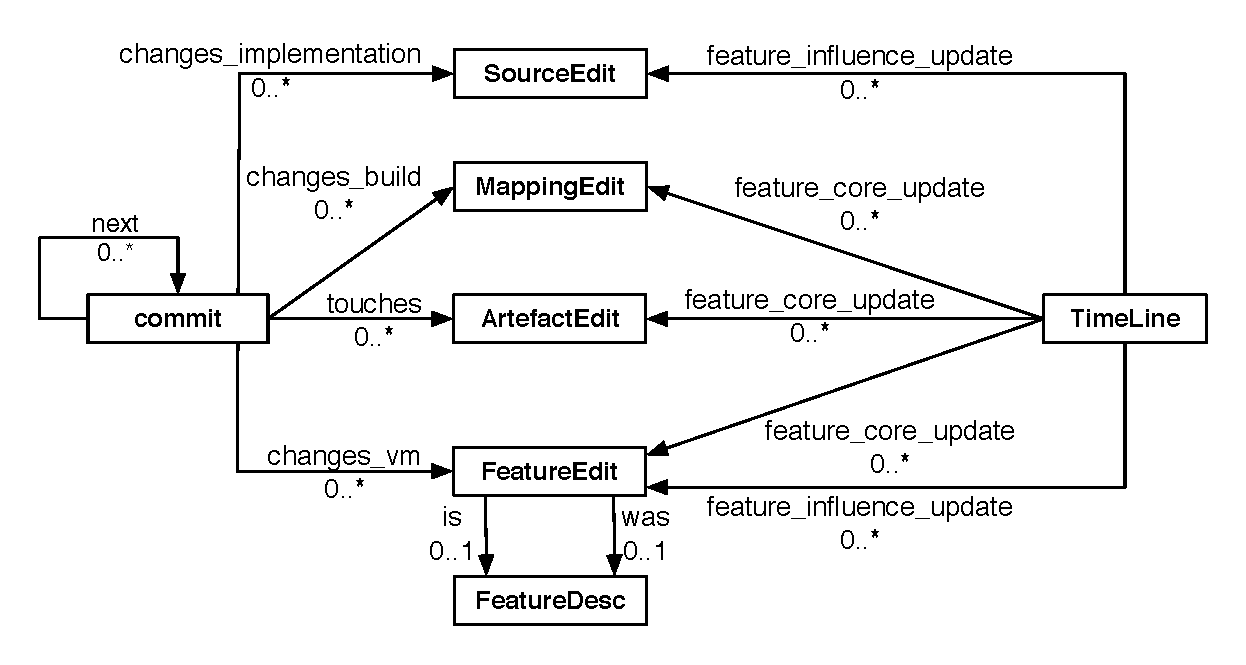
\includegraphics[scale=0.5]{change_model_new.eps}
	\caption{The FEVER change meta-model for feature-oriented change description}
	\label{fig:patch_change_model}
\end{figure}

For a commit in the repository we record the commit id (sha1) to link our data with the reference repository. 
We save the commit message which may contain information about the rationale of a change.
Finally, to keep track of who touches which feature, we record users-related information such as commiter and author of each commit.
\tabref{commit_attrs} summarizes the commit-related information stored in the FEVER database, examplified with the commit adding the 
``APDS9300'' feature.

\begin{table}[h]
\centering
\resizebox{\textwidth}{!}
{
\begin{tabular}{|l|l|l|}
\hline
Attribute 		& Details 										& Example\\
\hline
hash			& 10 first digits of the commit unique ID 		& 03eff7b60d \\
\hline
author			& author's name 								& Oleksandr Kravchenko\\
\hline
commiter 		& commiter's name 								& Jonathan Cameron\\
\hline
message 		& complete commit message, including sign-offs 	& iio: add APDS9300 ambilent light sensor driver (...)\\
\hline
time			& commit time 									& Sat Aug 03 19:40:37 CEST 2013\\
\hline
\end{tabular}
}
\caption{FEVER \textbf{Commit} entity attributes }
\label{commit_attrs}
\end{table}

\subsection{Variability Model Changes}

A \textbf{FeatureEdit} entity represents the change of one feature within the variability model performed in the context of a \textbf{commit}.
We are interested in the affected feature, as well as the change operation that took place (\textit{addition}, \textit{removal}, or \textit{modification} of an existing feature).
The \textbf{FeatureEdit} entity also points to a more complete description of the feature, \textbf{FeatureDesc} entities. 
\textbf{FeatureDesc} presents the feature as it ``was'' before the change (if existing)  and how it ``is'' after the edit operation (if existing).

In our example, the developer added a new feature, APDS9300, to the variability model.
The change that can be observed in the source control system is shown in \figref{fig:vm_change_diff}.

\begin{figure}[h]
\centering
	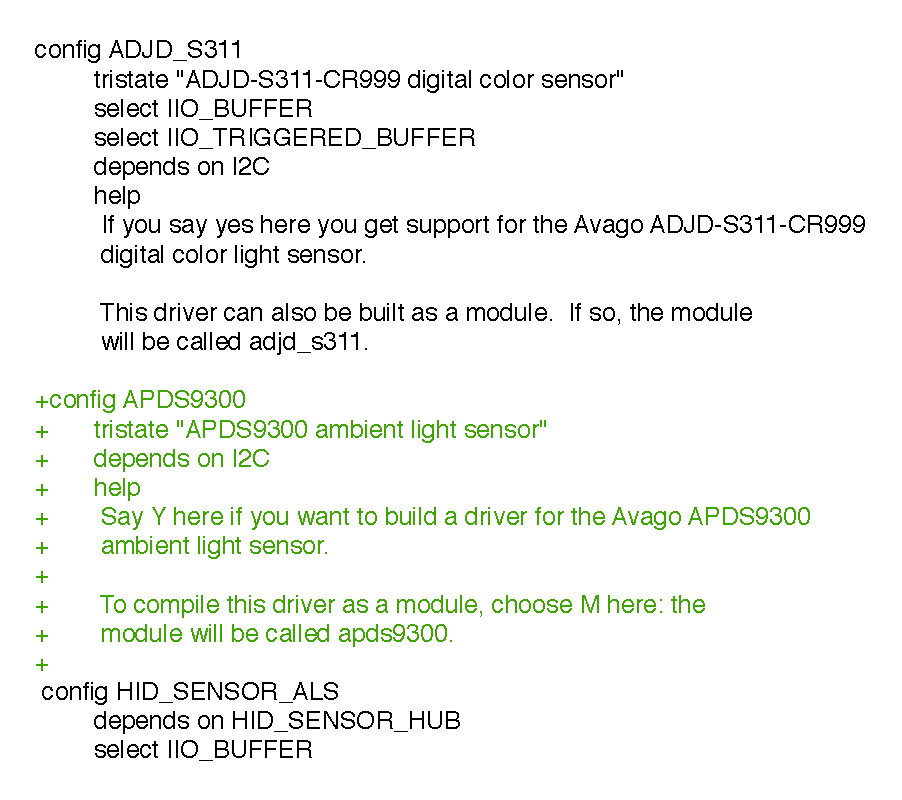
\includegraphics[scale=0.5]{VM_Diff_NewFeat.eps}
	\caption{Variability model change: addition of the feature APDS9300}
	\label{fig:vm_change_diff}
\end{figure}

The information recorded by FEVER on \textbf{FeatureEdit} entities are summarized in \tabref{featureedit_attrs}.
\begin{table}[h]
\resizebox{\textwidth}{!}
{
\centering
{
\begin{tabular}{|l|l|l|}
\hline
Attribute & Details & Example\\
\hline
name			& name of the touched feature & APDS9300 \\
\hline
change		& change operation affecting the feature  & ADDED\\
\hline
visibility	& feature visibility to user during configuration & visible\\
\hline
type &  type of the feature, defines its possible values & TRISTATE\\
\hline
\end{tabular}
}
}
\caption{FEVER \textbf{FeatureEdit} entity attributes }
\label{featureedit_attrs}
\end{table}

The possible values for the ``change'' attribute are: ``ADDED'', ``REMOVED'', or ``MODIFIED''.
The type attribute matches the configuration option type in the Kconfig language (``BOOLEAN'',``TRISTATE'', ``INT'', ``HEX'', or ``STRING'').
The feature is either ``visible'' or ``internal''.
Note that the type, and visibility information stored on the \textbf{FeatureEdit} entity correspond to the state of the feature after the edition takes place.
For additional information on the state of the feature before and after the change, one can refer to the \textbf{FeatureDesc} entities connected
to the \textbf{FeatureEdit} entity.

The \textbf{FeatureDesc} entity captures the information presented in \tabref{featuredesc_attrs}. 
\begin{table}[h]
\centering
\resizebox{\textwidth}{!}
{
\begin{tabular}{|l|l|l|}
\hline
Attribute & Details & Example\\
\hline
name			& name of the touched feature & APDS9300 \\
\hline
type 		& feature type &  TRISTATE \\
\hline
visibility 	& feature visibilty to the user during configuration & visible \\
\hline
depends on  & dependencies of the feature & I2C \\
\hline
selects 	    & the selected features & (none) \\
\hline
default values & default values, with conditions if any & (none) \\ 
\hline
\end{tabular}
}
\caption{FEVER \textbf{FeatureDesc} entity attributes}
\label{featuredesc_attrs}
\end{table}

For any feature change occurring at a variability model level, the change will be represented by a ``FeatureEdit'' entity, and at least one ``FeatureDesc'' entity in case of addition or removal,
and at most two in the case of the modification of an existing feature.


\subsection{Mapping Changes}

Regarding the evolution of the mapping, we are mainly interested in  the evolution of the mapping between feature and asset.
For this study, we consider the following types of assets: implementation artefacts, data artefacts, folders, and compilation flags.
The evolution of the mapping space is represented by \textbf{MappingEdit} entities characterized by:
the feature involved and the type of artefacts it is mapped to.
We describe the feature-mapping change operation (\textit{added}, \textit{removed}, or \textit{modified}),
referring to the association of a feature to any type of assets, and the change affecting the target within that mapping (\textit{added} or \textit{removed}).
Finally, if the asset is an artefact (file), then the change meta-model also includes the change to the artefact itself.
We can thus make the difference between a situation where a new mapping is introduced (\textit{addition} of a mapping with an \textit{added} target)
and an existing mapping being extended (\textit{modification} of a  mapping with an \textit{added} target).
If the asset is not an artefact (such as a folder or a compilation flag) the value of the ``artefact change'' attribute is set to ``NA''.

In our example, the developer adds a mapping between the newly created feature and a newly added file by
modifying an existing Makefile as shown in \figref{fig:mapping_change_diff}.
The information contained within the \textbf{MappingEdit} entity to represent this change are presented in \tabref{mapping_attrs}.

\begin{figure}[h]
\centering
	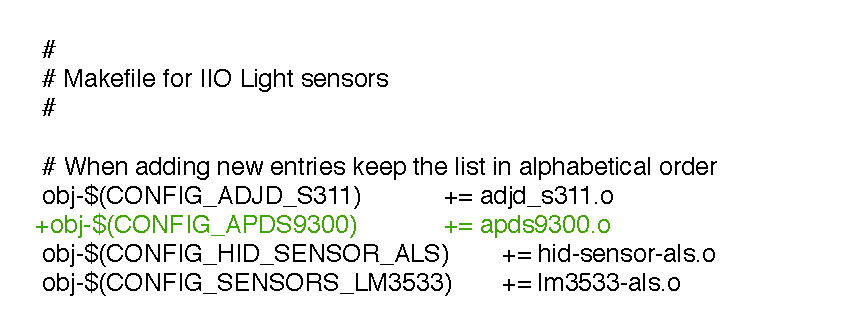
\includegraphics[scale=0.5]{Mapping_Diff_NewFeat.eps}
	\caption{Mapping change: introduction of a new association between feature and asset}
	\label{fig:mapping_change_diff}
\end{figure}

\begin{table}[h]
\centering
\resizebox{\textwidth}{!}
{
\begin{tabular}{|l|l|l|}
\hline
Attribute & Details & Example\\
\hline
type 		& element mapped to the asset &  FEATURE \\
\hline
feature		& name of the feature involved & APDS9300 \\
\hline
target		& target of the mapping & apds9300.o\\
\hline
target type	& type of the target (folder, flag, data, compilation unit)  & COMPILATION\_UNIT \\
\hline
mapping change  & change to the mapping of the feature  & ADDED \\
\hline
target change & change to the target entity within the feature's mapping & ADDED \\
\hline
artefact change	    & change to the artefact pointed to by the target & ADDED \\
\hline
\end{tabular}
}
\caption{FEVER \textbf{MappingEdit} entity attributes }
\label{mapping_attrs}
\end{table}

\subsection{Source Code Changes}

Feature related changes within source code, such as modifications to conditionally compiled blocks and feature references, 
are captured as \textbf{SourceEdit} entities.
Features in \#ifdef code block conditions and feature references within a given file are an indication 
that the behaviour of the feature mapped is configurable, and its exact behaviour is determined by other features.

Feature references are references to feature names within the code, meant to be replaced by the feature's value at compile-time.
Such references may only be \textit{added} or \textit{removed}.
In such cases, the \textbf{SourceEdits} entity contains the name of the affected feature and the change in question.

Conditionally compiled code blocks are identified by the conditions under which they will be included in the final product.
A change to such a block is represented by a \textbf{SourceEdit} containing the condition of the block, 
the change to the block itself (\textit{added, removed, modified}), and the change of the implementation within that block: 
\textit{added} if the code is entirely new, \textit{removed} if the whole block was removed, 
\textit{modified} when the changed block contains arbitrary edits, or finally \textit{preserved} if the code itself has not been touched.
An example of the code change is depicted in \figref{fig:src_change_diff}.

\begin{figure}[h]
\centering
	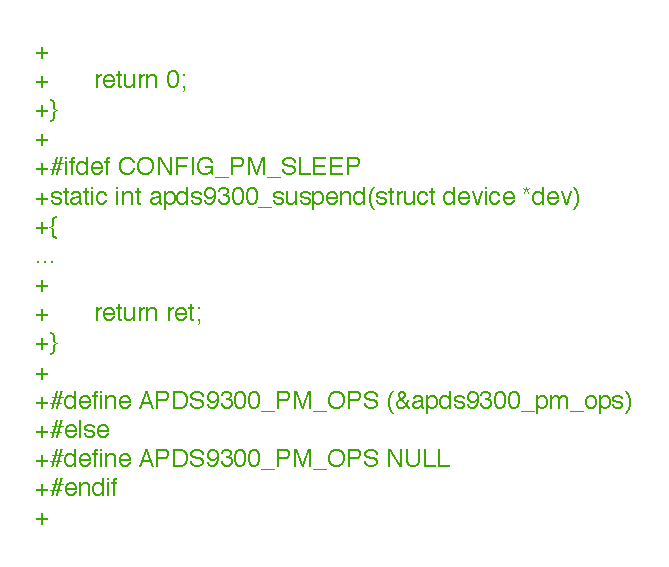
\includegraphics[scale=0.5]{Src_Diff_NewBlock.eps}
	\caption{Source change: addition of  conditionally compiled code blocks}
	\label{fig:src_change_diff}
\end{figure}

In our example, two code blocks are added. \tabref{sourceedit_attrs} presents the information we obtain
for the creation of the \textit{else} fragment of this change.
A similar entity is created for the first part of that new code block, the only different being the value of 
``interaction'' attribute which would reflect the condition of the first block, namely ``\textit{defined(CONFIG\_PM)}''

\begin{table}[h]
\centering
\resizebox{\textwidth}{!}
{
\begin{tabular}{|l|l|l|}
\hline
Attribute & Details & Example\\
\hline
Change 			& change to the code block itself, or the feature reference &  ADDED \\
\hline
Interaction		& presence condition of the block, or feature name for feature reference & !(defined(CONFIG\_PM\_SLEEP)) \\
\hline
Code Edit		& transformation of the code inside the changed block, ``null'' for references  & ADDED \\
\hline
\end{tabular}
}
\caption{FEVER \textbf{SourceEdit} entity attributes }
\label{sourceedit_attrs}
\end{table}

\subsection{TimeLines: Aggregating Feature Changes}

Changes pertaining to the same features are then aggregated into \textbf{TimeLine} entities.
A \textbf{TimeLine} entity aggregates all changes pertaining to a single feature in a number of commits - this includes
modification of artefacts mapped to the feature in question, FeatureEdit, MappingEdit or changes to conditionally compiled code blocks whose conditions refer to that feature.
For this study, we created \textbf{TimeLine} entities for entire releases.

We divide the types of changes that may affect a feature into two broad categories: 
\emph{core changes} and \emph{influence changes}.

A \emph{feature core update} indicates that the behaviour of the feature itself or its definition is being adjusted.
This comprises changes to the feature definition in the VM, changes to the mapping between the feature and assets,
and changes affecting assets mapped to that feature. 

A \emph{feature influence update} indicates that the feature is playing a role in the behaviour of another feature.
This occurs in two contexts: in the source code, as part of a \textbf{SourceEdit}, or in the variability model as 
part of a \textbf{FeatureEdit}. For instance, in the first case, Feature B plays a role in the implementation of A if we can find
an \#ifdef block refering to B in a source file mapped to Feature A. Similarly, Feature B plays a role in the definition of feature A
if Feature B appears anywhere in the definition of A in the variability model (as part of a default value, depends or select statement or any other attribute).

\figref{fig:commit_overview} depicts all entities and relationships used to describe the changes occurring in single commit
03eff7b60d. This is a partial view of the complete database. When fully expanded, the ``PM\_SLEEP'' \textbf{TimeLine} points to any
\textbf{Edit} entity which describe changes to the ``PM\_SLEEP'' feature across an entire release.
By navigating through those relationships, one can easily find what transformation occured on each feature and retrieve contextual information 
regarding this change.

\begin{figure}[htb]
	\centering
	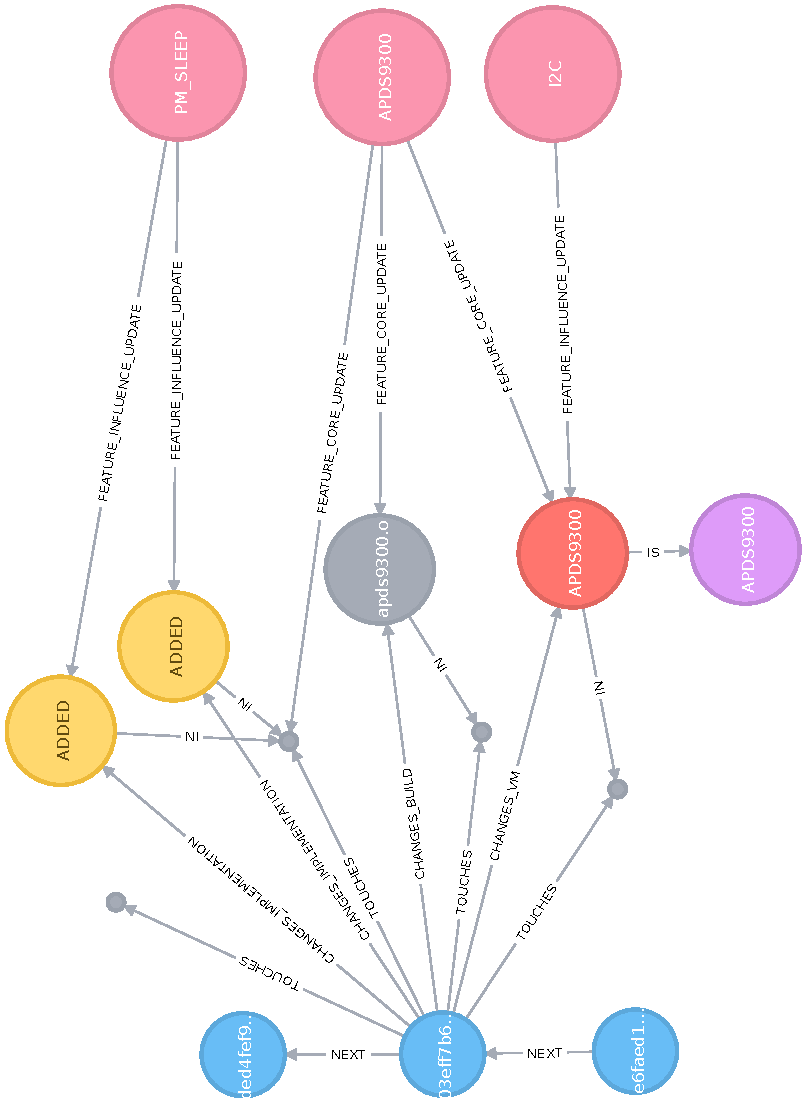
\includegraphics[scale=0.55,angle =-90, natwidth=450,natheight=500]{full_commit.pdf}
	\caption{FEVER representation of commit 03eff7b60d - all entities and relationships. For readability purposes, \textbf{ArtefactEdits} are
	represented by small unlabelled gray dots. From top to bottom, they represent edits to the following files: a documentation file, 
	the source file containing the  behavior of feature APDS9300, 
	the Makefile containing the new mapping, and the Kconfig file containing the new feature declaration.
	On the left hand side, we see three commits. On the right hand side, we see three feature \textbf{TimeLine} entities, one for each feature that was adjusted in the commit. In the middle, from top to bottom we see two source edits (labeled ``ADDED'') indicating that two \#ifdef blocks were added, one \textbf{MappingEdit}, labeled ``apds9300.o'', then a \textbf{FeatureEdit} entity indicating taht feature APDS9300 was changed, and a \textbf{FeatureDesc} entity containing a detailed description of how the feature ``is'' after the change.}
	\label{fig:commit_overview}
\end{figure}

\begin{sloppypar}

In \figref{fig:commit_overview}, three \textbf{TimeLine} entities are depicted in pink, on the right hand side of the diagram, annotated with the feature name.
The first one relates to the feature that was introduced. We can see that
the ``APDS9300'' node is connected to the \textbf{FeatureEdit}, in red in the diagram marked with the feature name ``APDS9300'', the \textbf{MappingEdit} in gray annotated with the name of the changed target (apds9300.o), and an \textbf{ArtefactEdit} (represented by a small gray dot for visibility purpose) with a ``feature\_core\_update'' relationship.
The connection between the \textbf{TimeLine} for this feature and the \textbf{ArtefactEdit} is deduced from the \textbf{MappingEdit}:
because the new mapping assigns this artefact to feature APDS9300, then the introduction of this artefact is a ``core'' update of this feature.
The APDS9300 \textbf{TimeLine} connects the different changes occurring in three different types of artefacts, all related to the same operation: the addition of a feature.

We can also see that a \textbf{TimeLine} for feature PM\_SLEEP is present and connected to two \textbf{SourceEdit} entities.
This indicates that, at the creation time, the driver APDS9300 interacts with the power management ``sleep'' feature,
and this interaction occurs in two different code blocks.
Finally, a TimeLine for feature I2C point to the FeatureEdit introducing feature APDS9300.
Note that, APDS9300 depends on I2C, and that relationship is new. For that reason, in this commit
the influence of feature I2C was changed, however its implementation was not modified.

\end{sloppypar}

It is important to note that changes are extracted on an ``per artefact basis''.
This means that entities being moved within the same artefacts (a feature in a Kconfig file, or a mapping in Makefile) will be seen as modified. 
However, if an entity is moved from one artefact to another, this is captured as two separate operations: a removal and an addition, and as such, two \textbf{Edits} entities. 
Those two \textbf{Edit} entities are linked together by a \textbf{TimeLine} entity, referring to the modified feature.


\section{Populating FEVER}
\label{sec:extraction}

\subsection{Overview}

\begin{figure}[h]
	\centering
	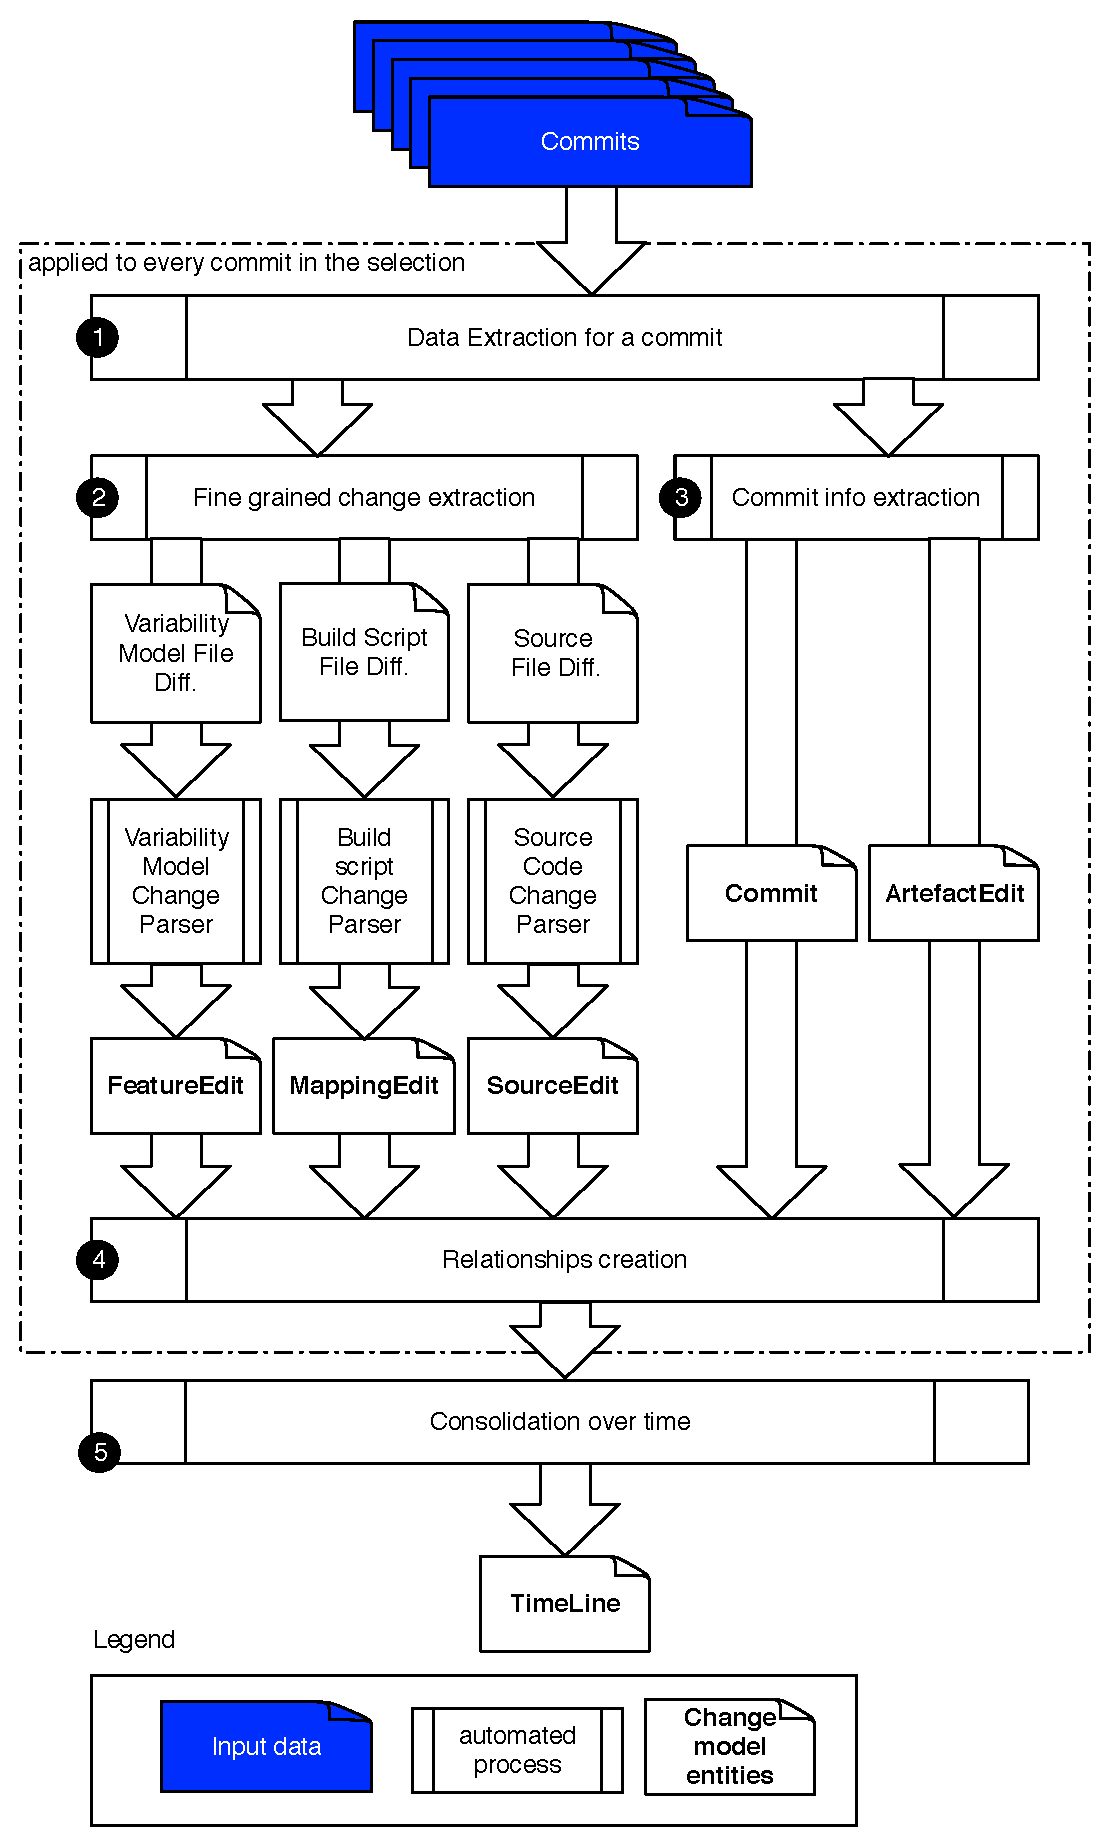
\includegraphics[scale=0.35]{extraction_overview.eps}
	\caption{Overview of the FEVER change extraction and consolidation process}
	\label{fig:overview}
\end{figure}
The FEVER approach starts from a set of commits and outputs an instance of the FEVER change model covering the given commit range.
\figref{fig:overview} presents an overview of the change extraction process.
From the initial set of commits, FEVER first analyses each commit separately, and then consolidates the extracted change information.
For each commit, Steps 1 to 4 are executed as follows:

\textit{Step 1} is the identification of the touched artefacts and the dispatch to the appropriate change parser.
In the Linux kernel, artefact types are characterized by naming conventions and file extensions using the mapping presented in \tabref{file_heuristics}.
Compared to our previous work \citep{dintzner_fever:_2016}, we adjusted our artefact identification heuristics regarding source files, with a more restrictive expression on ``.S'' files (rather than ``.S*'').
We also include binary files (libraries), which were previously not taken into account.

\begin{table}[h]
\centering
{
\begin{tabular}{|l|l|}
\hline
Artefact type & Expression used for identification\\
\hline
V.M. file	& ``Kconfig.*'' \\
Build file	& ``Makefile.*'',``Kbuild.*'',``Platform.*'' \\
Source file & ``*.c'', ``*.h'', ``*.s'', ``*.S''\\
Binary file & ``*.dll'',``*.so'',``*.a'',``*.lib''\\
Data file	& ``*.dts'',``*.dtb''\\
\hline
\end{tabular}
}
\caption{Artefact types: regular expression used to identify the different types of artefacts}
\label{file_heuristics}
\end{table}

\textit{Step 2} performs the artefact-specific data extraction processes. 
The next subsections (\secref{sec:vm_model},\secref{sec_mapping_model}, and \secref{sec_impl_model}) 
detail  the process for each type of artefact, but all of them follow the same general steps.
First FEVER rebuilds a model of the artefact as it was before the change, 
and a second one representing the same artefact after the change.
Then, FEVER uses the EMF Compare\footnote{\url{http://wiki.eclipse.org/EMF\_Compare}} infrastructure to identify 
the differences between the two versions of the model.
EMF Compare identifies the differences between the two models, and extracts them in terms of the EMF meta-model.
FEVER then translates those changes into the different \textbf{Edit} entities depending on the artefact type.
The reconstruction of the models, and the identification of changes (based on EMF Compare results)
are based on heuristics and assumptions on the structure of the artefacts.
We provide an evaluation of the accuracy of those heuristics in \secref{sec:evaluation}.

\textit{Step 3} is the extraction of changes in artefacts for which we do not extract detailed changes.
This includes only commit-related information from which we create a \textbf{commit} entity, 
and ``untyped'' artefacts (\ie documentation, or scripts), represented by \textbf{ArtefactEdit} entities.

In \textit{Step 4}, FEVER creates the relationships between \textbf{Edit} entities, the \textbf{Commit}, and \textbf{ArtefactEdit}.

\textit{Step 5} of our approach consists in creating entities and relationships spreading beyond single commits:
``next'' relationships among commits to keep track of the sequence of changes, and feature \textbf{TimeLine} entities 
with their respective relationships to edit entities.
This is done by navigating through every commit, and identifying touched feature(s), 
creating if necessary a new \textbf{TimeLine} entity and the appropriate relationships between 
the \textbf{TimeLine} and relevant edits.

We continue this section by describing the heuristics we used to extract feature related changes. 
Those heuristics are based on multiple sources of information, namely the work of Neves et al. \citep{neves_safe_2015}, the work of Passos et al. \citep{passos_coevolution_2015}, 
the Linux official documentation,  and finally the authors' expertise \citep{passos_coevolution_2015,dintzner_analysing_2015}.


\subsection{Extracting Variability Model Changes}
\label{sec:vm_model}

We describe in this section the artefact-specific change extraction process (Step 2 in \figref{fig:overview})
that takes place when a commit contains changes to the variability model of the system.
\begin{figure}[h]
	\centering
	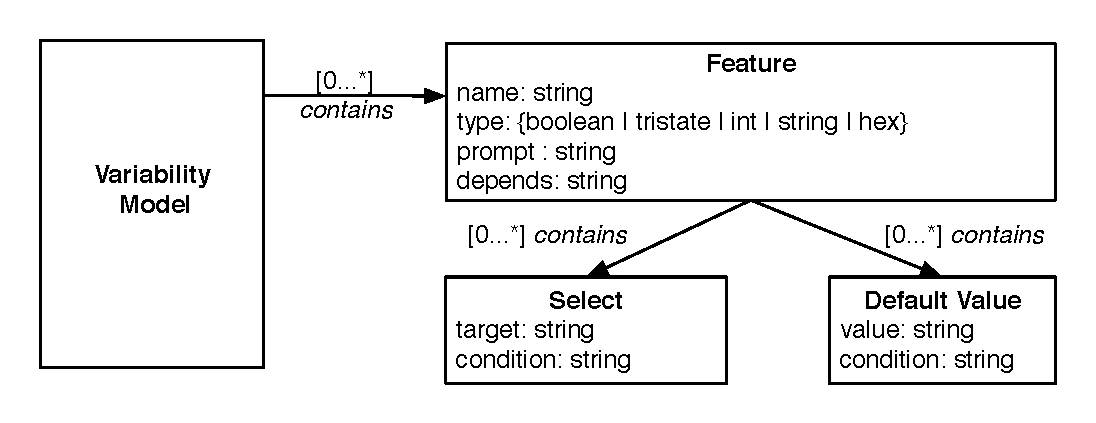
\includegraphics[scale=0.40]{EMF_VM_Model.eps}
	\caption{Representation of the variability model used for change extraction}
	\label{fig:vm_for_diff}
\end{figure}

The characteristics of the changed features that we focus on are their type (Boolean or value-based) and the change
affecting the feature.
We first reconstruct two instances of the VM depicted in \figref{fig:vm_for_diff} per VM file touched, 
one representing the VM before the change, the other after the change.
If, like in the case of the Linux kernel, the VM is described in multiple files,
we reconstruct the parts of the model described in the touched files, \ie the model we rebuild is always partial with respect to the complete Linux variability model.
The extraction process follows the FMDiff approach \citep{dintzner_analysing_2015}, including the usage of ``dumpconf''. 
This tool takes as an input a Kconfig file and translates it into XML. 
``dumpconf'' is designed to work on the complete Kconfig model, where the different files are linked together with a ``source'' statement, similar to \#include in C.
To invoke ``dumpconf'' successfully on isolated files, we remove the ``source'' statements as a pre-processing steps.
``dumpconf'' also affects the attributes of features, and the details of the change operation are described in \citep{dintzner_extracting_2013}.
We use this XML representation of the Linux VM to build the model shown in \figref{fig:vm_for_diff}.

We then use EMF Compare to extract the differences and compile the information in a \textbf{FeatureEdit} entity. 
To successfully compare two model instances, FEVER needs to provide EMF with the capability to determine that
two features in the two model instances are the same entity.
For this, we rely on the feature name as a unique identifier during the model comparison phase.

We attach to this entity the snapshot of the feature as it was before and after the change in \textbf{FeatureDesc} entities.
If the feature is new, respectively deleted, we do not create a ``before'', respectively ``after'', \textbf{FeatureDesc} entity.
As mentioned, the ``source'' statement in the Kconfig language is used to link Kconfig files together.
Such statements can be used in combination with other constructs, such as menus, or ``if'' blocks.
In this situation, the presence condition of the menu, or the condition of the ``if'' blocks, in practice
applies to all features within ``sourced'' file, and any of the files it might ``source'' itself.
By working on a file level (touched Kconfig file), FEVER will not capture such complex changes.

With respect to our previous work \citep{dintzner_fever:_2016}, we now handle cases where two features within the same file have the same name.
Whereas the previous heuristic yielded a number of false positive, such cases are now handled by suffixing feature names by an index if a feature name is encountered
twice (or more) when rebuilding the EMF model we use for change extraction.


\subsection{Extracting Mapping Changes}
\label{sec_mapping_model}

We describe in this section the artefact-specific change extraction process (Step 2 in \figref{fig:overview})
that takes place when a commit contains changes to the mapping between features and assets.

\begin{figure}[h]
	\centering
	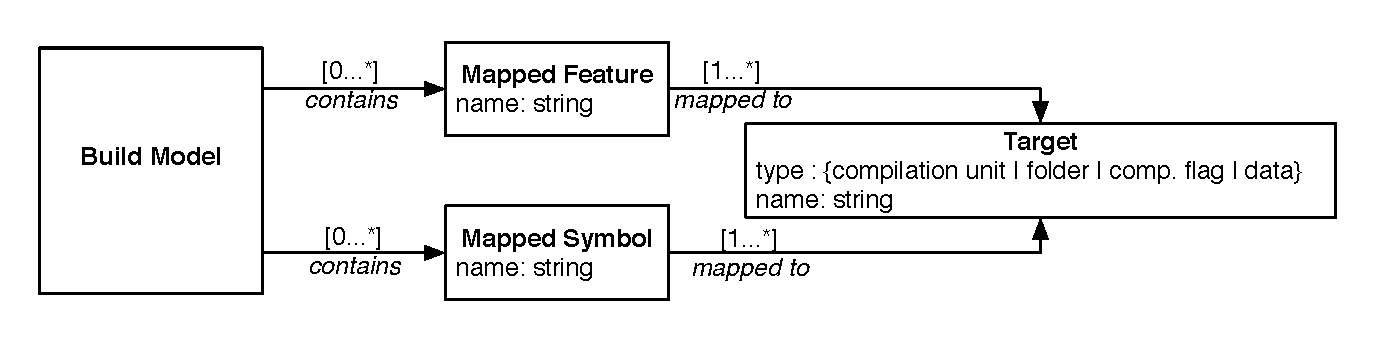
\includegraphics[scale=0.40]{EMF_Build_Model.eps}
	\caption{Representation of the feature-asset mapping used for change extraction}
	\label{fig:mapping_for_diff}
\end{figure}

Similar to the extraction of VM changes, \textbf{MappingEdit} entities are created based on the differences 
of reverse engineered models of a Makefile, before and after the change.
We use the model shown in \figref{fig:mapping_for_diff}.

The model contains a set of features and symbols mapped to targets. 
``Symbol'' refers to any variable mapped to any assets which is not a feature. 
We identify feature names in Makefiles by their prefix ``CONFIG\_''.
We scan the Makefiles and extract pairs of symbols by searching for assignment operators (``+='' and ``:=''). 
We consider that the symbol on the left hand side is mapped to the symbol on the right hand side (target).

To determine the type of a targeted asset, we use the following rules:
Compilation unit names finish with either ``.o'',``.c'' or ``.h''; 
mapped data artefacts in the Linux kernel are identified by the extensions ``.dts'', ``.dtb''; 
compilation flags either start by the follwing strings ``-D'', ``-L'', ``-m'',  or ``-W'', ``-I'', ``-f''.
We identify folder names by ``/'', or single words, not containing any special characters nor spaces.

Makefiles may contain lists of assets that will be included in the compilation 
as soon as the Makefile itself is included.
Those assets are assigned to Makefile variables whose names depend on the implementation of the build process.
In the Linux kernel, those are identified by \footnote{https://www.kernel.org/doc/Documentation/kbuild/makefiles.txt}:
``obj-y'',``lib-y'',``ccflags-y'',``asflags-y'', and ``ldflags-y''.
When we find assets associated with such variables, we map them to a temporary variable, using the following convention: we use the
key word ``guarded\_'' and append the name of folder containing the Makefile.
We later use this naming convention with the extracted information on features mapped to folders 
to assign the changes of such Makefile variables to the appropriate feature(s).

When features are found as part of ``ifeq'' or ``ifneq'' statements, we consider that they are mapped to any targets contained within their scope.
In Listing \ref{modular_makefile_ifdef}, both CONFIG\_OF and CONFIG\_SHDMA will be mapped to the compilation unit ``shdma.o''.

We also resolve aliases within Makefiles.
An example of an alias is presented in \listingref{modular_makefile_ifdef}, 
where feature CONFIG\_BLK\_DEV\_SWIM is mapped to the alias ``swim\_mod.o'' referring to two compilation units ``swim.o'' and ``swim\_asm.o''.
The association between ``swim\_mod'' and the two compilation units is done the last line of the listing.
We identify such aliases based on the naming convention : name of the object file appended by ``-y''.
Note that there are no concrete artefact corresponding to ``swim\_mod'' by itself in the Linux source tree.
This step is performed as a post-processing step for each build model instance, 
and is based on heuristics, also evaluated in \secref{sec:evaluation}.

\begin{lstlisting}[language=diff, caption=Example of an ``ifeq'' statement and aliases used in Makefiles, label=modular_makefile_ifdef]
ifeq ($(CONFIG_OF),y)
   shdma-$(CONFIG_SHDMA) += shdma.o
endif
obj-$(CONFIG_BLK_DEV_SWIM)	+= swim_mod.o
swim_mod-y	:= swim.o swim_asm.o
\end{lstlisting}

Finally, FEVER uses a Linux specific heuristic for mapping files contained within specific folders.
Part of the mapping between feature and folder is done using variable names, and dynamic path reconstruction.
In general, FEVER does not attempt to recover this mapping, but for a specific set of folder in the Linux kernel, namely the architecture folders,
this mapping is important.
Upon compilation, the chosen hardware architecture of the kernel forces the selection of a given subfolder of the ``./arch'' folder.
There is no explicit declarations of that mapping in any Makefile (it uses variables and name reconstruction).
For this reason, FEVER assumes that any file within the ``arch/x86'' folder maps to feature ``X86'' if no other mapping is found.
The accuracy of this heuristic to recover the link between features and artefacts is evaluated in the next section
as the \textit{feature-file mapping} change attribute.

Our model reconstruction is based on heuristics and therefor do not take into account all the possible constructs used in the Linux kernel to link artefacts to features, however, FEVER focuses on those mentioned above.
The constructs that FEVER does not capture are based on variable name manipulation, to build artefacts names (e.g. folder names, or file names),
or combining lists of artefacts together.
Then, as mentioned in \secref{sec:background}, the exact mapping between features and files
is the result of a complex Makefile hierarchy. 
By focusing on the mapping as described in a single Makefile, FEVER only captures a part of the presence condition
of each file.

Once the two instances of the model are reconstructed, we use EMF Compare to extract the differences between them,
giving us the list of feature mappings that were added or removed in that commit.
For the comparison of two instances of our mapping model, we use the name of features as unique identifiers.

From the earlier version of this work \citep{dintzner_fever:_2016}, we now capture mapping between features and more artefacts, and our coverage of compilation flags is more comprehensive.
In addition, we now take into account the changes to the mapped artefact as well. We can now determine whether a change in the mapping is also associated with changes to the mapped artefacts themselves. 
Doing so, we can differenciate cases where a feature change involves a new mapping to a new artefact, and cases where the new mapping points to a pre-existing artefact.


\subsection{Extracting Implementation Changes}
\label{sec_impl_model}

We describe in this section the artefact-specific change extraction process (Step 2 in \figref{fig:overview})
that takes place when a commit contains changes to the implementation (source code).

\begin{figure}[h]
	\centering
	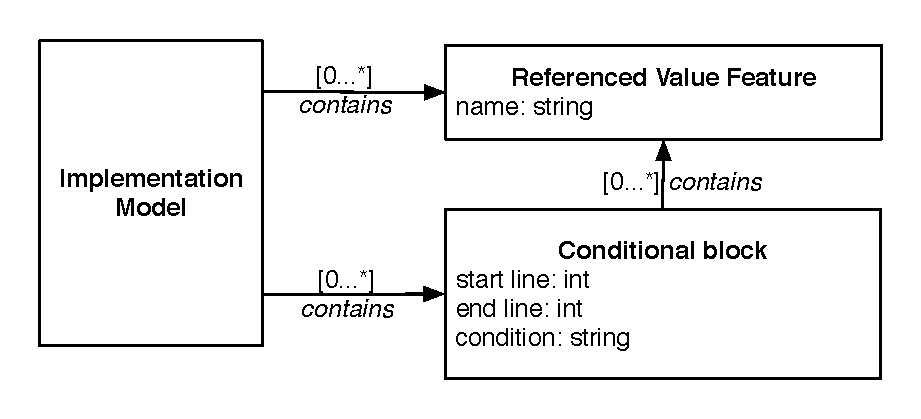
\includegraphics[scale=0.40]{EMF_Source_Model.eps}
	\caption{Representation of the feature-asset mapping used for change extraction}
	\label{fig:source_for_diff}
\end{figure}

At the implementation level, we consider changes to \#ifdef blocks and changes to feature references in the code, as presented in \secref{sec:background}.
To extract those changes, we rebuild a model of each implementation file in its before 
and after state following the model presented in \figref{fig:source_for_diff}.

To rebuild the models, we rely on CPPSTATS \citep{liebig_analysis_2010} to obtain 
starting and ending lines of each  \#ifdef block as well as their guarding condition. 
It should be noted that CPPSTATS provide the condition of each block by taking into account nesting.
In practice, if a block with condition B is nested inside a block with condition A, CPPSTATS will 
report two blocks, one with condition A and one with condition ``A\&B''.

In the model, code blocks and their \#else counter-parts are captured as two distinct entities.
``Referenced value features'' are obtained by scanning each modified source file looking for the usage 
of the ``CONFIG\_'' string outside of comments and \#ifdef statements.
Note that we report reference changes once per feature and per file.

We then use EMF Compare to compare the two models and build the \textbf{SourceEdit} entities.
For this comparison, FEVER needs to use a unique identifier for each code block contained within a source file. 
The condition on a block may not be unique, and hence cannot be used to uniquely identify a block in 
two versions of the source model.
The location of the block within the file may change during a commit without the block being changed itself
(\ie if code is added or removed above it).
FEVER uses a combination of the condition of the block combined with its content (the actual code)
as a unique identifier.
This proved to be an efficient technique, but in the context of the Linux kernel a number of files 
contain identical code blocks, with the same block condition.
While this may seem surprising, one may consider a logging mechanism: if the logger feature is selected, write an entry in the log file.
This might be repeated in multiple functions in a file. 
As a result, the EMF comparison process cannot correctly identify changed blocks and returns a number of false positive changes.
To compensate for this, we add indices to the identifier of code blocks when we find such duplication.

We determine the code changes occurring inside \#ifdef blocks to compute the value of the ``code edit'' attribute of 
\textbf{SourceEdit} entities.
This is performed as a separate step, once we found the changed code blocks.
We extract from the commit the diff of the file in the ``unified diff'' format, and identify which lines of code where modified.
We compare this information with the first and last lines of each modified code block to determine 
which code block is affected by the code changes.

FEVER extracts and records changes to all conditionally compiled code blocks - whether features play a role
in their presence condition or not.
Changes to code blocks that are not tied to any feature will be captured as \textbf{SourceEdit}, but
such entities will not be linked to any \textbf{TimeLine} in the next step of our process.

By comparison with our previous work \citep{dintzner_fever:_2016}, we enhance the source change extraction process by taking into account cases
where code artefacts contain identical code blocks, containing identical code. Such situations caused errors
during the EMF comparison process and are dealt with as explained in this section.


\subsection{Change Consolidation and TimeLines}
\label{sec:timelines}

The final step consists in the creation of feature \textbf{TimeLine} entities and relate them to the appropriate entities.
We create such entities for every feature touched affected by any change in any \textbf{Edit} entity.
We apply the following strategy: 
\begin{itemize}
\item if a feature is touched in the VM, mapping or source file, the corresponding \textbf{Edit} entity is associated with a \textbf{TimeLine} with a ``core update'' relationship.
\item if a feature A is added from another feature B's attribute (as part of a constraint), then the \textbf{FeatureEdit} entity representing this change is connected to the feature \textbf{TimeLine} with an ``influence update'' relationship if feature A did not participate at all in the definition of B before the change.
\item if a feature A is removed from another feature B's attribute (as part of a constraint), then the \textbf{FeatureEdit} entity representing this change is connected to the feature \textbf{TimeLine} with an ``influence update'' relationship if feature A no longer participate at all in the definition of B after the change.
\item if a feature is part of the condition in a \textbf{SourceEdit} entity, the \textbf{SourceEdit} is connected to one \textbf{TimeLine} entity per feature present in the condition with an ``influence update'' relationship;
\item if an artefact is touched, it is linked to the \textbf{TimeLine} entity of the feature to which it is mapped with a ``core update'' relationship. This is done for each feature mapped to the file.
\end{itemize}

In order to map file changes to features, we need to know the mapping between features and files.
Note that FEVER only focuses on mapping changes, leaving us with a gap with respect to mappings that are not touched.
As a result, many files, whose mapping has not evolved would not be mapped - wrongly - to any features.
To compensate for this, we create a snapshot of the complete mapping based on the state of the artefacts on the first commit of the commit set.
To support systems which do not follow Linux naming convention (the CONFIG\_ prefix used in Makefile and the source code), 
we also extract the list of features present at the beginning of the studied time-frame.
For both the initial feature list and initial mapping, 
we rely on the FEVER parser to obtain the information by invoking it for every Kconfig file and Makefile present in the system. 

We then run through all commits, starting from the leaves in a breadth-first manner, creating or updating \textbf{TimeLine} as necessary,
and updating the known mapping between files and features as we encounters \textbf{MappingEdits}.
Note that there may be more than one initial commit in a set: we have to consider branches as well. In our experiment we usually have
one initial commit of the release itself, and the different branches that have not yet been merged.\footnote{the list of commit is obtained using the following Git log command, asking for all commit reachable from the last considered commit and not accessible from the first commit of the release - i.e.: \textit{git log v3.7...v3.8}} 

Some files in the Linux kernel cannot be mapped directly to features. 
This concerns mostly header files, contained in ``include'' folders.
``Include'' folders do not contain Makefiles, which prevents direct mapping between features and such artefacts.
Moreover, such files are included in the compilation process on the basis that they are referenced by implementation files (\#include statement), 
which by definition bypasses any possible feature-related condition.
For those reasons, we do not attempt to map such files to features.
They are, however, highly conditional, and often contain many \#ifdef statements, which we track.


\section{Evaluating FEVER with Linux}
\label{sec:evaluation}

The FEVER change extraction process is based on heuristics and assumptions about the structure of the artefacts. 
Those heuristics affect the model build phase and the comparison process - the mapping between EMF model changes and higher-level
feature oriented changes. 
It is then important to evaluate whether the data captured by FEVER reflects the changes that are performed by developers
in the source control system. 

The objective is two-fold. First, we aim at evaluating how the changes to the heuristics impacted the accuracy of the FEVER approach.
Secondly, we aim at providing a complete evaluation of the FEVER approach and its accuracy, 
including all new change attributes, against a larger and more representative set of commits as before.

Throughout this section, we consider that a FEVER change description is ``accurate'' if the changes
performed by developers are captured correctly by FEVER as described in the previous section.
We evaluate the accuracy of the approach in terms of precision and recall with respect to changes 
performed by developers on the observed artefacts.

With this work, we improved on the existing FEVER prototype \citep{dintzner_fever:_2016} in several ways.
\secref{sec:approach} described the FEVER approach with its improvements.
From the initial version of this work, we improved the following aspects of the approach:
\begin{itemize}
\item heuristics for code reference identification
\item heuristics for code changes within modified code blocks
\item heuristics for asset-feature mapping identification (compilation flag, default list, and artefact extensions management)
\item the build change model to support more types of artefacts (namely data artefacts)
\item the build change extraction to include artefact changes when describing mapping changes
\item the timeline model to include ``influence updates'' on feature changes
\end{itemize}

With those changes, FEVER captures more information than before, and should be able
to capture previous information more accurately. 
This leads us to formulate the first research question driving this evaluation:
\begin{framed}
RQ1: To what extent is the new version of FEVER more accurate in capturing feature-related changes?
\end{framed}

However, the enhancements of FEVER also include the addition of new information regarding feature-related changes.
The overall accuracy of the tool, should also be evaluated. We propose to answer the following research question:
\begin{framed}
RQ2: To what extent does the improved FEVER data match changes performed by developers?
\end{framed}

To assess whether the FEVER data matches the content of commits, we perform here a two-steps evaluation. 
First, we apply FEVER on the commits used in \citep{dintzner_fever:_2016} and compare the results obtained
during the first evaluation of FEVER and the improved algorithm. 
Then, we perform a second, entirely new evaluation on two different releases using a different
heuristic to select commits.

For both steps, the evaluation is performed manually and consists in comparing the content of the FEVER database
with changes performed by developers.
We first present how this comparison is performed. Then, we present the results of the replication 
of the evaluation and finally present the results of the evaluation on the new set of commits. 

\subsection{Evaluation Method}

The objective is to evaluate the accuracy of the heuristics and the model comparison process used for artefact change extraction 
and the change consolidation process.
To do so,  we manually compared the content of the FEVER dataset with the information that can be obtained from Git, using the GitK user interface.
GitK provides a view of the list of changed files, the chunked of modified texts in each of them, with an adjustable number of lines of context for each chunk.
The number of line of context provided for each chunk is particularly relevant for us since conditionally compiled code blocks can be large, and identifying in which block a change occurred may require a very large context (up to the complete file).
The evaluation was performed by the main author of this paper.

For a set of commits, we checked that the different \textbf{Edit} entities and their attributes can be explained by the changes observed in Git.
Conversely, we ensured that feature-related changes seen in Git have a FEVER representation.

To facilitate the evaluation, we first dump the FEVER representation of the selected commits in a file, containing all captured 
information for those commits (all spaces, all files, all edit entities and their relationships). 
We obtain this information simply by querying the FEVER database. 
We then proceed with the comparison by types of artefacts - first by checking if all files seen as touched in FEVER are indeed touched in the commit, and we continue until all changes have been verified.

At variability model level, we checked whether the features captured by FEVER as added, removed, or modified are indeed
changed in a similar fashion in the Linux Kconfig files.
We pay special attention to specific cases such as features being moved inside files - which may or may not result in actual changes to the feature,
but surely are not addition nor removal scenarios and must be recorded by FEVER as a modification of an existing feature.

Regarding mapping changes, we checked that the pairing of features and files is accurate and that the type of targeted artefact
is also correct.
Special consideration was given to the validation of the mapping between features and assets (artefacts or compilation flags).
During the validation, we assess both which features are being mapped and what they are being mapped to. 
Although we should note that a transformation associating a single feature to multiple different artefacts is recorded by FEVER
as a three multiple associations, and are taken as such during the evaluation.

The mapping between features and files may be the results of complex Makefile constructs and may 
be distributed over several files through inclusion mechanism.
FEVER only takes into account a number of such constructs as mentioned in \secref{sec:approach}, but not all possible ones.
In cases where a mapping change can be observed in a Makefile, but FEVER does not report
any change, we checked in the Makefile hierarchy if a feature should have been mapped to that change.
If, during the manual inspection, we reached the root folder of the Linux file hierarchy and
we have not encountered any explicit declaration of a link between the changed mapping and any feature, 
we considered that this change could not have been mapped by FEVER, and FEVER should not report any feature-related mapping change.
For instance, a developer modifies ``./mm/Makefile'' (memory management), and adds a compilation unit to the ``obj-y'' variable.
We see that the inclusion of the file ``./mm/Makefile'' is not conditioned by any feature in the root ``./Makefile'' of the kernel source tree.
Hence, we consider that FEVER cannot map this mapping change to any feature, and should not report it.
During the evaluation, if an artefact is not assigned to a feature in FEVER and we cannot manually find
which feature it should be assigned to following the methodology presented above, we consider that the FEVER output is correct.
We emphasize that FEVER will still report that the Makefile has been touched in the form of a \textbf{ArtefactEdit},
but no \textbf{MappingEdit} entity should be present.

At the code level, we checked that the blocks seen as touched are indeed touched, and we compared the condition of each block.
Then, by inspecting the patch, we validated that the code changes within the blocks were correct.

Regarding \textbf{TimeLine} entities, we did not check whether all relevant changes in all commits were indeed gathered into \textbf{TimeLine} entities.
We made the assumption that if \textbf{TimeLine} entities were properly linked in the commits we checked, then
the algorithm is correct, and the check on the complete release is therefor unnecessary.
We also kept track of the commits for which all extracted information is accurate, giving us an overview of the accuracy on a commit basis.



\subsection{Replication}

In our previous work \citep{dintzner_fever:_2016}, we evaluated our tool as follows.
Using FEVER, we extracted feature changes from release 3.12 and 3.13 of the Linux kernel, and randomly extracted 150 commits from each release (out of 11,907 and 13,288 respectively).
The selection of commits in those two releases was performed as follows:
we randomly selected 50 commits touching at least the variability model, 50 among the commits touching  at least the mapping,
and 50 touching at least source files.
Those three sets are non-overlapping.
So the creation of three different sets ensures that our random sample covers all three spaces.
During the evaluation, we ignored merge and release tag commits.

To evaluate our improved algorithm, we performed the same analysis over the same set of commits using the enhanced FEVER prototype and compared the
results obtained with what was previously established. 
\tabref{review_attrs} presents a comparison between the previous 
precision and recall obtained on change attributes as well as the precision and recall for the new algorithm.


\begin{table}[t]
\centering
\resizebox{\textwidth}{!}
{
\begin{tabular}{|l|r|r|r||r|r|r|}
\hline
& \multicolumn{3}{c|}{Reference algorithm \citep{dintzner_fever:_2016}} & \multicolumn{3}{c|}{Current algorithm} \\
\hline
Attribute & Sample & Precision (\%) & Recall (\%) & Sample & Precision (\%) & Recall (\%)\\
\hline
VM operations 							&  &  & & & & 					  		\\
change: \textit{added} 					&  208 & 100 & 100 & 206 & 100  & 99		\\
change: \textit{removed}					&  73  & 100 & 100 & 74  & 100  & 100	\\
change: \textit{modified}				&  140 & 80  & 100 & 138 & 81.4 & 98.6	\\
\hline
Mapping operations						&  &  & & & & 							\\
target: \textit{folder}					& 17 & 100 & 94 & 17 & 100 & 100			\\
target: \textit{compilation unit}		& 437 & 100 & 98  & 430 & 100 & 99.8		\\
target: \textit{compilation flag}		&  10 & 67 & 60 & 14 & 100  & 100		\\
mapping change: \textit{added}	    		& 278 & 99  & 97 & 271 & 98.9 & 98.9		\\
mapping change: \textit{removed}  		& 84 & 100 & 95 & 133 & 100 & 100		\\
mapping change: \textit{modified} 		& 98 & 100  & 98 & 68 & 98.6 & 100		\\
target change: \textit{added}			& 326 & 99  & 97 & 328 & 98.2 & 97.9		\\
target change: \textit{removed}			& 133 & 100 & 97 & 139 & 100 & 100		\\
\hline
\textit{file-feature mapping} 			& 622  & 81  & 97 & 728 & 93.4 & 92.6	\\
\hline
Source operations						&  &  & & & & \\
block change: \textit{added}				& 381 & 81 & 97 & 321 & 98.7 & 92.6 		\\
block change: \textit{removed}			& 229 & 100 & 99 & 230 & 100 & 97.8 		\\
block change: \textit{modified} 			& 237 & 97  & 99  & 233 & 96.3 & 100 	\\
code change: \textit{added}  			& 365 & 99  & 97  & 307 & 99.0 & 98.4 	\\
code change: \textit{removed}			& 195 & 99  & 99  & 190 & 96.4 & 98.4 	\\
code change: \textit{edited}				& 237 & 96  & 99  & 236 & 95.9 & 100 	\\
code change: \textit{preserved}			&  46 & 32  & 83  & 45  & 93.2 & 91.1	\\
reference change: \textit{added}			& 6 & 100   & 83	  & 106  & 100 & 100		\\
reference change: \textit{removed}		& 7 & 88    & 100 & 5 	 & 83.0 & 100	\\
\hline
TimeLine 								& 743 & 93 & 98  & 11225 & 95.5 & 97.5\\
\hline
\end{tabular}
}
\caption{Comparison of accuracy of the initial FEVER heuristics \citep{dintzner_fever:_2016} with its new version.}
\label{review_attrs}
\end{table}

In addition to the information presented in the table, our evaluation showed that 
the percentage of commits for which FEVER correctly extracted all change attributes
increased from 82.7\% to 85.3\%.

Let us first discuss the differences in terms of sample change between the two evaluations. 
We note that between the two evaluations, few sample size are exactly the same.
For instance, the first evaluation recorded 208 added features, but the second one found a total of 206. 
The evaluation process being inherently manual, it is reasonable to observe slight differences (as in the variability model changes for instances).
However, variation of sample size is more significant for the following attributes: 
feature-file mapping, block changes added, added code, added references, and timelines. 
Regarding the feature-file mapping, the new version of FEVER attempts to resolve the mapping of more files 
- rather than focusing only on source code. 
Previously, FEVER did not do so for files located within an ``include'' folder (at any level of its path).
Changes to files in folder such as ``arch/.../include'' are now mapped.

The variation in our sample of ``block changes: added blocks'' and ``code change: added code'' are related. 
During the first evaluation, we found 381 added code blocks (block changes: added blocks) with 365 occurrences of new code blocks containing only new code (code change:added code),
while during the second evaluation the number of added code blocks dropped to 321, and the number of code blocks with added code
dropped to 307.
The difference between the two values stems from changes obtained from a single commit. A file with the extension ``.S\_shipped'' containing
a large number (60+) of added interactions was included in the initial evaluation. 
We adjusted the algorithm to identify files, enforcing strict file extension (.S), hence the file was ignored
during the second evaluation. This results in less added code blocks, and the less added code blocks containing only new code.
While this raises the question of which artefacts one should consider during the experiment, it does not
undermine the ability of FEVER to capture accurately code changes from within a well defined set of artefacts.

The number of added references increased significantly between the two evaluations.
Once again, explanation for this difference is contained within a single commit\footnote{206f060c21} where
a hundred features are added, and then referenced in the code. During the first evaluation, 
those references where incorrectly identified as local macros by the tool and the reviewer, and not noted as added references.
During the second review, with the updated algorithm, the references were correctly identified by FEVER as feature references.
A deeper analysis of the code and the related artefacts showed that those were indeed feature references
and should be recorded as such.

Finally, with the improved approach,\textbf{TimeLines} now may be created as the result of a feature relationship change.
Since this was not taken into account during the first evaluation, the number of \textbf{TimeLines} obtained with the improved algorithm (11,225)
is \textit{de facto} larger than during the first evaluation (743).
The conditions under which we create \textbf{TimeLines} are presented in \secref{sec:timelines}. In that list, the points two and three, on
feature relationship changes were previously not recorded. However, the 743 \textbf{TimeLines} initially recorded are a subset of the 11,225 
\textbf{TimeLines} observed during the replication.

Despite those differences, the results in \tabref{review_attrs} indicate improvement of the
accuracy of most change attributes related to mapping and code changes.
The most significant being the detection of preserved code inside changed code blocks (from a precision of 32\% to 93.2\%)
and the detection of changes to compilation flags during mapping evolution (from a precision and recall of 67\% and 60\% to 100\%).
Code change capture was improved by avoiding false positives when multiple code blocks were identical.
The detection of compilation flag changes was improved by capturing changes to compilation flags not mapped ``directly'' to a feature, but indirectly (the flag is mapped to an internal variable and will be activated when a guard feature is selected).

With this information we can answer our first research question, RQ1: To what extent is the new version of FEVER better at capturing feature-related changes?
\begin{framed}
The overall accuracy of FEVER slightly improved (by 2.6\%), while the ability to 
capture certain change attributes increased significantly (by more than 30\%).

The changes to the heuristics used by FEVER lead to an improvement over its previous version.
\end{framed}

While this increases our confidence in FEVER's ability to capture changes, the improved algorithm
allowed us to capture change in artefacts and feature relationships 
that were not taken into account before - hence, not covered in this comparison.
Moreover, we used for this comparison the same set of randomly selected commits as in our previous work \citep{dintzner_fever:_2016}.
However, the methodology used to build this set did not allow for commits not affecting any feature to be included
in the evaluation, which, in our opinion created a bias in the initial evaluation. 
We continue the evaluation of FEVER by performing a complete evaluation, including new attributes 
on a more complete and different set of randomly selected commits.

\subsection{Evaluation on a New Set of Commits}
\label{sec:new_eval}
The results of the previous sub-section highlight improvements on the ability of FEVER to capture certain types of changes.
However, we extended the change model to capture additional change information, as presented in 
the beginning of this section.

To evaluate the improved FEVER algorithm, we extended the evaluation of the data used in the replication 
presented above (300 commits) to cover the additional changes and created a new dataset from two releases using a different random selection approach (510 additional commits).
For the additional dataset, instead of three groups of commits affecting different spaces, 
we randomly selected commits from five different groups: 51 commits not affecting any artefact, 51 commits affecting arbitrary artefacts, 
51 commits affecting at least the variability model, 51 commits affecting at least the mapping, and finally 51 commits affecting
at least code blocks, for a total of 255 commits per release.
With this approach, we ensure that every commit within the FEVER database may be selected.
Consequently, the complete dataset used for this evaluation is comprised of 810 commits, from 4 different releases
(150 commits from release 3.12, 150 commits from release 3.13, 255 commits from release 3.14, and 
finally 255 commits from release 4.2).

FEVER does not capture changes inside merges. The rationale behind this decision is to avoid
capturing changes multiple times: once when they are implemented by their original authors, and 
possibly a second time if the merge operation results in a conflict (same file modified twice).
During our evaluation, we checked whether some information was missed by skipping merge commits altogether.
We used the following methodology: we inspected a subset of the merge commits and checked that all changes that occurred can be
found within the parent commits - i.e. all modifications pre-existed, they are simply integrated together.
We identify ``new content'' in merge commits by using the following ``git log'' command to visualize the changes: 
\begin{quote}
git log <commit\_hash> -p --cc 
\end{quote}

The ``-p'' option displays the patch, and "-cc" displays the patch ``diff'' from all parents simultaneously.
Using this view of the patch, we searched for content added or removed from all parents. 
Practically, this amounts of searching for lines in the ``diff'' where the number of ``+'' or ``-'' symbols
at the beginning of modified lines of text equals the number of parents.\footnote{https://git-scm.com/docs/git-log}
Given that FEVER omits merge commits, any of such change is accounted for as a false negative for the relevant change attribute
during the evaluation.
\tabref{complete_review} summarizes the results for the 4 datasets, comprised of a total of 810 commits.

\begin{table}[t]
\centering
\small
{
\begin{tabular}{|l|r|r|r|}
\hline
Attribute & Population & Precision (\%) & Recall (\%) \\
\hline
VM operations 							&  &  &   				\\
change: \textit{added} 					&  309 & 100  & 98.7		\\
change: \textit{removed}					&  88  & 100  & 98.9 	\\
change: \textit{modified}				&  293 & 89.8 & 98.6		\\
\hline
Mapping operations						&  &  & 					\\
target: \textit{folder}					& 52  & 100 & 98.1		\\
target: \textit{compilation unit}		& 735 & 99.3 & 95.6 		\\
target: \textit{compilation flag}		& 32  & 100 & 100 		\\
target: \textit{data}					& 61  & 100 & 100 		\\
mapping change: \textit{added}	    		& 506 & 98.4  & 95.1 	\\
mapping change: \textit{removed}  		& 201 & 100 & 90.0 		\\
mapping change: \textit{modified} 		& 180 & 97.7  & 92.8		\\
target change: \textit{added}			& 644 & 98.7  & 94.6		\\
target change: \textit{removed}			& 224 & 99,1 & 100		\\
artefact change: \textit{added}	    		& 366 & 98.2  & 91.5		\\
artefact change: \textit{removed}  		& 113 & 99.0 & 89.4		\\
artefact change: \textit{modified} 		& 31 & 100  & 80.6		\\
artefact change: \textit{untouched}   	& 290 & 88.7  & 92.4		\\
artefact change: \textit{NA}   			& 82 & 100  & 98.8		\\

\textit{file-feature mapping} 			& 1650  & 95.1  & 93.5	\\
\hline
Source operations						&  &  & \\
block change: \textit{added}				& 656 & 99.4 & 93.5	 \\
block change: \textit{removed}			& 355 & 100 & 97.2	 \\
block change: \textit{modified} 			& 529 & 95.6  & 99.6	 \\
code change: \textit{added}  			& 583 & 99.1  & 97.9	 \\
code change: \textit{removed}			& 271 & 97.0  & 96.7	 \\
code change: \textit{edited}				& 556 & 95.3  & 99.3	 \\
code change: \textit{preserved}			&  124 & 95.7  & 88.7 \\
reference change: \textit{added}			& 117 & 99.2   & 100  \\
reference change: \textit{removed}		& 9 & 69.7    & 100   \\
\hline
TimeLine 								& 2367 & 97.1 & 97.5  \\
\hline
\hline
Correct commits							& 810 & \multicolumn{2}{c|}{87.2\%} \\
\hline
\end{tabular}
}
\caption{FEVER change extraction accuracy evaluated on 810 commits}
\label{complete_review}
\end{table}

The results show that, for a majority of attributes (26 out of 27), FEVER precision and recall is at least of 88\%.
On the other hand, we note that detection of reference changes can be problematic.
During this evaluation, we found two cases where developers created local variables
(using the \#define C directive) whose name matched feature naming convention (CONFIG\_ prefix).
This explains the lower precision, but FEVER still exhibit for this change a high recall of a 100\%  
when capturing removals of feature references.

If we compare the results obtained during the complete evaluation with the results obtained during the replication of our first evaluation, we note
that, for a number of change attributes, the accuracy dropped by small yet noticeable amounts (for precision and recall alike).
This is due to the increase in our sample size and a more thorough sampling approach. We considered for the complete evaluation a larger,
more representative sets of commits in the Linux kernel as explained in \secref{sec:new_eval}.
As we observe more changes, we see more commits containing changes deviating from what FEVER is able to parse.
We can say that, given the increase in our sample and the a more balanced sampling techniques, this evaluation is more precise than what 
we had provided in the past. 

With this information we can now answer our second research question, RQ2: To what extent does the new version FEVER data match changes performed by developers?

\begin{framed}
The results showed that the data collected by the new version of FEVER matches the changes performed by developers in 87\% or more of the commits.
The newly included change attributes (artefact changes, ``data'' artefact types) are captured with a high accuracy (of at least 80\%).
\end{framed}

Those results give us confidence on the viability of the FEVER approach, and in the quality of the extracted data.
We proceed to explore usages of the dataset, before continuing with an exploratory study of co-evolution of artefacts
in the context of feature evolution in \secref{sec:coevolution}.

%\subsection{Discussion on FEVER Accuracy}
%\label{sec:threats_fever}
%
%Before moving on to explore the data collected using the FEVER approach, let us discuss the 
%accuracy and limitations of the approach itself.
%
%\textit{Limitations.}
%Our evaluation shows that FEVER captures feature-related changes with a relatively high accuracy (87,2\% of commits extracted completely correctly).
%However, FEVER does not capture all feature related information in all artefacts.
%Because FEVER operates on a file-basis, with a text-based parser, certain constructs in the variability model or the mapping
%are not captured. 
%The limitations of FEVER for each space are mentioned in the relevant sub-sections of \secref{sec:approach}.
%
%\textit{Internal validity.}
%To extract and analyze feature-related changes, FEVER uses model-based differencing techniques.
%We first rebuild a model of each artefact, and then perform a comparison.
%The construction of the model relies on heuristics, which themselves work based on assumptions on the structure of the touched artefacts - 
%whether they be code, models, or mappings.
%For this reason, information might be lost in the process.
%To guarantee that the data extracted by FEVER do match what can be observed in commits, 
%we performed a manual evaluation, covering change attributes our approach currently consider.
%The evaluation showed that a large majority of the changes are captured accurately, with a precision and recall of at least 80\%.
%This gives us confidence in the reliability of the data.
%
%Using manual analysis for validation purposes is inherently fault prone.
%The difference in populations of changes observed between the initial and enhanced versions of the tool
%does highlight this.
%For this evaluation, the manual review of commits was performed twice - for the entire dataset, leaving a small
%time gap (between 2 days and a week) between the two evaluation rounds.
%While the errors identified in the initial evaluation lead to a significant update for some change attributes (namely ``added feature references'' in the code), evaluation errors occurred in less than 5\% of the commits.
%
%The evaluation of the new FEVER heuristics, compared to its previous version, highlights significant improvement of accuracy on specific change attributes. 
%In particular the capture of code block changes with preserved code block improved from  a precision of 32\% to 93.3\%. 
%Moreover, the added change attributes (namely artefact changes, additional artefact type, and \textbf{TimeLine} relationships to \textbf{FeatureEdit}) were captured with a good precision and recall (at least 80\%).
%
%Because the FEVER approach is based on heuristics, it is neither sound nor complete. 
%But for more than 80\% of the extracted commits, the data does reflect changes performed by developers.
%While this may be a limitation when searching for very specific changes, with specific change attributes, 
%overall trends and statistics done over the course of a release reflect developer's activities on features in the Linux kernel
%with sufficient accuracy to draw conclusions from it.
%
%\textit{External validity.}
%We devised our prototype to extract changes from a single large scale highly variable system, namely the Linux kernel. 
%In that sense, our study is tied to the technologies that are used to implement this system: the Kconfig language, 
%the Makefile system and the usage of code macros to support fine-grained variability.
%The models used for comparison do contain attributes that are very tightly related to the technology used in the Linux kernel.
%However, there are several other systems using those very same technologies, such as aXTLs\footnote{aXTLS: http://axtls.sourceforge.net/index.htm} and uClibc\footnote{uClibc: https://uclibc.org/}, on which our prototype 
%- and thus our approach - would be directly applicable.
%
%For other types of systems, one would need to adapt the model reconstruction phases depending on the system under study.
%If we consider another operating system such as eCos\footnote{eCos: http://ecos.sourceware.org/}, one would need to rebuild the same change model from features
%described in the CDL language\footnote{CDL : http://ecos.sourceware.org/ecos/docs-3.0/cdl-guide/reference.html} instead of Kconfig.
%Concretely, this amounts to creating a CDL parser capable to build the same EMF variability model representation used in this work to initiate the comparison process.
%Attributes such as default value, select, or visibility would be relevant, and the ``select'' attribute can simply be left empty.
%A similar effort would be necessary to consider systems using the Gradle build system\footnote{Gradle: https://gradle.org/}, rather than the Make system.
%However, the change model, based on an abstract representation of feature changes,
%should be sufficient to describe the evolution of highly variable systems, regardless of the implementation technology.
%Moreover, our work shows that model-based differencing is a suitable approach to extract feature related changes
%from heterogeneous artefacts in large scale systems.
%
%Our work focuses on build-time variability, constructed around the build system and 
%an annotative approach to fine-grained variability implementation (\#ifdef statements).
%While we believe that the change model may be useful to describe runtime variability,
%the extraction process is not suitable to extract feature mappings from the implementation itself at this time.
%We cannot extend this work to runtime variability analysis without further study.

%intro

\section{FEVER usage scenarios}
\label{sec:in_practice}
In this section, we illustrate how using FEVER or the data collected using the approach can be of use 
to developers, maintainers and researchers in the scenarios \textbf{S1} to \textbf{S4} mentioned in the \secref{sec:Introduction}.

The FEVER data is stored in a Neo4j graph database.\footnote{http://neo4j.com/} 
Every entity of the FEVER change meta-model is a node of the graph, and the relationships are edges.
Data types are represented using node labels, and attributes are stored as node properties.
The queries presented in this section are written in the Cypher query language.\footnote{http://neo4j.com/docs/stable/cypher-query-lang.html}
It is understood that, in a practical situation, an integration with development tools would be more suitable than 
relying on direct Cypher queries.

\subsection{FEVER for Software Development Activities}

In scenario \textbf{S1}, we consider the work of a release manager
building the release notes. He is interested in highlighting important features, 
and matching those to the commits that participated in their implementation.
The release notes of Linux v3.13 \footnote{http://kernelnewbies.org/Linux\_3.13}
mention the following change ``add[s] option to disable kernel compression'' with a single commit.
Looking at the commit, we know that a new configuration option named ``KERNEL\_\-UNCOMPRESSED'' is introduced.
We can check this with FEVER by querying the commits 
associated with the \textbf{TimeLine} of ``KERNEL\_\-UNCOMPRESSED'' as follows:
\vspace{-.5ex}
\begin{verbatim}
match 
(t:TimeLine)-[]->()<-[]-(c:commit)
where t.name = "KERNEL_UNCOMPRESSED"
return distinct c; 
\end{verbatim}
\vspace{-.5ex}
This query returns two commits. The first commit (id:69f055) mentioned in the release note
is associated with a \textbf{FeatureEdit} entity denoting the addition of a feature.
The second commit (id:2d3c62), occurring a few days later, is also associated with a \textbf{FeatureEdit} entity, but, surprisingly, \emph{removes} the feature.
A check in release v3.14 showed that the feature was never re-introduced. This means that the release notes written by the 3.14 release managers were, in fact, incorrect.
We argue that a dataset such as FEVER would provide release manager with more accurate information on changes that were performed by developers and may have prevented this erroneous entry in the release notes.

In scenario \textbf{S2}, a developer is about to introduce a new driver for a touch-screen 
supporting the power management ``SLEEP'' feature.
The developer might want to know how such support was implemented in other drivers and compare it with its own implementation.
Using FEVER, he queries the database for commits where a new feature (f1) is added (fe.change =``ADDED''),
and interacts with a second feature (f2) whose name is ``PM\_\-SLEEP'' as follows:
\vspace{-.5ex}
\begin{verbatim}
match (f1:TimeLine)-[:FEATURE_CORE_UPDATE]->
             (fe:FeatureEdit)<-[]-(c:commit),
 (c)-[]->()<-[:FEATURE_INFLUENCE_UPDATE]-(f2:TimeLine)    
where f2.name = ``PM_SLEEP''  and fe.change = ``ADDED''
return f1,f2, distinct c;
\end{verbatim}
\vspace{-.5ex}

When ran against database containing commits of release 3.14 of the Linux kernel, this query returns ten results, giving the name of the
newly introduced features, and the commits in which those changes occurred.
Among the results, the developer might notice that feature ``TOUCHSCREEN\_ZFORCE''
and might consider using this as an example to drive his own development.

In this scenario, FEVER is used as a ``recommender'' system to guide the implementation of a new component.
Relying on previous activities to guide further development is a common approach to ease software evolution.
We can name Hipikat \citep{cubranic_hipikat:_2003}, CodeBook \citep{begel_codebook:_2010} as tools aiming for such facilities.
However, such approaches do not take into account the deep structure of the implementation
which FEVER does by breaking artefact changes by feature.
This degree of granularity is particularly interesting for variant-rich system.
For such scenarios, we believe that the information obtained by FEVER would be a valuable addition to existing approaches such as CodeBook,
rather than a replacement.


FEVER can also be of use in our third scenario \textbf{S3} in the context of bug triaging.
Let us consider the bug \#928561 reporting issues with keyboards mentioning that ``\textit{multimedia and macro keys are not working}''.\footnote{https://bugzilla.redhat.com/show\_bug.cgi?id=928561}
The bug report author provide traces and logs pointing to issues with the Linux Human Interface Devices (HID) subsystem.
This issue was fixed by and the patch was introduced in the  kernel in release 3.12.
In the FEVER database for release 3.12, we run the following query to see who among the commit authors committed
the most changes affecting HID related features.
\vspace{-.5ex}
\begin{verbatim}
match (c:Commit)-->()<--(t:TimeLine)
	where t.name=~"(?ism).*HID.*" 
	return distinct (c.author), count(c) 
	order by count(c) desc;
\end{verbatim}
\vspace{-.5ex}
The name of the developer who analyzed and fixed the issue comes first in the results, with 22 commits affecting ``*HID*'' features - 
among which one corresponds to the patch fixing  the keyboard issue.
In second place, we find an official maintainer for three of kernel subsystems with  17 commits, followed by another official maintainer 
for two HID related subsystems and the name of a Linux branch manager with 16 commits each affecting such features.
It is interesting to note that the names of the developers who fixed the issue in question 
are not present in the official maintainers list of the kernel for releases 3.11 nor 3.12. 
Through this scenario, we suggest that the FEVER database can be of use to identify feature expertise,
and possibly facilitate bug triaging \citep{matter_assigning_2009}.
A maintainer in charge of bug triage may use a simple query with information on potentially faulty features
to find which developers can provide insight on an issue or even fix it.

The number of bug reports, and the number of developers makes appropriate bug assignment to developers difficult.
To alievate some of those issues, several approaches have been designed to facilitate the identification of experts capable of fixing a bug \citep{ahsan_automatic_2009,matter_assigning_2009}.
Most of those solutions rely on previous fixes to determine, based on bug report content, who is the most likely to be able to provide an answer to a bug report.
What we propose is to take into account a feature-based expertise, and relate the bug report content with specific features, in order to determine
who is the best suited to fix bugs related to that feature.
This provides an additional type of information, based on fine-grained artefact changes, which can be particularly useful for artefacts at the limit 
of a subsystem where more than one team may be considered as potential fixers.
We do not claim that FEVER could replace existing approaches, but feature-related evolution information could be added to increase the accuracy
of existing techniques.

\subsection{FEVER for Software Engineering Research}

In scenario \textbf{S4}, a researcher in the domain of evolution of highly variable software systems
is interested in the typical structure of feature related changes.
For instance, he would like to observe the occurrences of the introduction of abstract features, in the sense of Thuem et al. \citep{thuem_reasoning_2009}: a feature only exists in the VM.
Using FEVER, we can identify the introduction of such features with this query:
\vspace{-.5ex}
\begin{verbatim}
match 
 (t:TimeLine)-[:FEATURE_CORE_UPDATE]->(f:FeatureEdit)
where 
 not (t)-[:FEATURE_CORE_UPDATE]->(:MappingEdit)
 and not (t)-[:FEATURE_CORE_UPDATE]->(:ArtefactEdit)
 and not (t)-[:FEATURE_INFLUENCE_UPDATE]->(:SourceEdit)
 and f.change="Add"
return t
\end{verbatim}
\vspace{-.5ex}
In release v3.13, this query returns 42 features. 
Because \textbf{TimeLine} entities are regrouping changes across spaces and commits,
we know that those 42 features are indeed abstract, and this is not the result
of a developer who first modified the variability model and in a later commit adjusted the implementation.
The addition of an abstract feature has not yet been described as a co-evolution pattern, and further analysis 
is necessary to fully describe such changes. 
Nonetheless, this illustrates how FEVER can be of use to discover patterns or identify instances of known patterns.
An earlier version of FEVER was used by Sampaio et al. to facilitate the identification of instance of changes affecting certain spaces
in the context of their work on safe evolution templates \citep{sampaio_partially_2016}.

In scenario \textbf{S5}, we consider the work of a researcher focusing on variability related bugs \citep{abal_42_2014} and bug prediction \citep{giger_comparing_2011}.
The data captured by FEVER may reveal information on features involved in bug-fixing commits.
A basic approach would consist in using regular expression on commit messages to identify bug-fixing commits.
Using this, one can identify features involved in bug-fixing commits using the following query:
\vspace{-.5ex}
\begin{verbatim}
match (c:commit)-->()<--(t:TimeLine)
	where not c.message =~ "(?ism).*copyright notices.*" 
			and c.message =~ "(?ism).* bug.*" 
			or c.message =~ "(?ism).* error.*" 
			or  c.message =~ "(?ism).* fix.*" 
			or c.message =~"(?ism).* revert.*" 
return t.name, count(distinct c);
\end{verbatim}
\vspace{-.5ex}
We note that Tian et al. devised a methodology to identify bug-fixing commits in the Linux kernel \citep{tian_identifying_2012}.
Combining such an approach with FEVER should yield more accurate results than the query presented here.
However, with such a simple query, one can identify which features are more error-prone than others.
It would be interesting to see if the number of features involved in a commit influences
the bug-proneness of commits.

Finally, the data provided by German et al. \citep{german_continuously_2015} can be used to track commits over time and across repositories.
Combining this information with the FEVER database would allow us to track feature development across Git repositories, 
and observe how the Linux community collaboratively handles the development of inter-related features.

The implementation of variant-rich system is known to be challenging. Features and their relationships, if misunderstood, can lead to issues such as dead code,
invalid products, or compilation errors.
To mitigate such problems, researchers have to identify the issues, find a way to fix them, and apply them on a number of cases for validation.
We argue here that tools such as FEVER are a convenient way of identifying what changes occurred in commits with respect to features.
Once a researcher has found a scenario where the studied error occurs, one can easily find other scenarios, with similar changes, and observe if the error occurred there as well.
FEVER by itself cannot mitigate such a problem, but constitutes a way to facilitate research in such a domain: by easing the search for a problematic situation, and providing a  quantitative estimate of the occurrences of problematic evolution scenarios.

Given the current accuracy of the FEVER prototype (85\%), a manual review of the changes is necessary to guarantee that the retrieved
changes are all correct. However, it is sufficient to reduce efficiently the number of commits that must be reviewed, and provide a solid starting point
for further manual analysis, as was done by Sampaio et al. \citep{sampaio_partially_2016}.

Conversely, should a developer run a query on FEVER and get no results, there is a small chance that FEVER may have failed to extract such changes (false negative).
In such a situation, the developer might have to rely on Git query instead, but FEVER already provides some information:
the type of change sought by the developer is not common, or the implementation used to support those specific features/constructs are
not what is commonly used in the Linux kernel.











\section{Co-evolution in Linux}
\label{sec:coevolution}

In this section we explore the data collected by FEVER over 15 releases of the Linux kernel.
Given the relatively high accuracy of the approach established in \secref{sec:evaluation}, 
we can rely on FEVER data to explore co-evolution of artefacts in the context of feature evolution in the Linux kernel.

The state of the art on feature-oriented co-evolution of artefacts in highly configurable software systems
focused on specific changes \citep{passos_coevolution_2015,neves_safe_2015,neves_investigating_2011}.
Those studies were performed using manual analysis. While those provide relevant and important 
knowledge on change scenarios, little information can be found on their occurrence 
in large systems. 
In this section, we report on an exploratory study of the feature-oriented co-evolution of artefacts in the Linux kernel. 

We argue that quantitative information on the frequency of co-evolution over the evolution of a complex system
would allow tool developers and researchers to determine how relevant the support of co-evolution for the evolution of such systems is.
How often is co-evolution occurring, and how many authors actually face co-evolution during their development tasks?
What percentage of the touched features actually evolve in multiple variability spaces? And when they do, which spaces 
are more frequently involved? 
Should a developer provide tool support for co-evolution, and what should be its main focus to help in a majority of cases? 
This leads us to formulate the following two research questions: 
\begin{itemize}
\item RQ3: To what extent do artefact in different variability spaces co-evolve during the evolution of features?
\item RQ4: To what extent are developers facing co-evolution over the course of a release?
\end{itemize}

With the first question, we can obtain an estimate of how likely co-evolution is from a technical perspective.
If a feature evolves during a release, how likely is it that this evolution will imply the modification of multiple types of artefacts?
With the second question, we aim at estimating the potential audience for tools and techniques
targeting co-evolution issues.
Provided a simple and efficient method can be devised to guarantee correct feature-oriented co-evolution
of artefacts, what percentage of the development team would actually benefit from it?

To put our results into perspective, we first provide our readers with
general information on the evolution of the Linux kernel as captured by FEVER over the studied
period of time.
The dataset collected with FEVER covers 15 releases of the Linux kernel, starting at v3.9 (April 2013 - first extracted commit) until v4.4.(January 2016 - last extracted commit).
A release of the Linux kernel lasts for approximately six weeks.


\begin{table}[h]

\centering
\begin{adjustbox}{width=\textwidth}
\begin{tabular}{|l|r|r|r|r|r|r|r|}
\hline
Release & 3.10 & 3.11 & 3.12 & 3.13 & 3.14 & 3.15 & 3.16 \\
\hline
Number of commits	& 14737 & 11851 & 11906	& 13288	& 13415	& 14871	& 13830	\\
Number of authors	& 1433	& 1304  & 1362  	& 1400	& 1481	&1535	& 1513	\\
Number of features	& 12511	& 12603	& 12780	& 13022	& 13134	& 13297	& 13453	\\
Number of timelines	& 5208	& 4397	& 4424	& 4581	& 4503	& 4960	&4099	\\
\hline
\end{tabular}
\end{adjustbox}

\vspace{5mm}
\begin{adjustbox}{width=\textwidth}
\begin{tabular}{|l|r|r|r|r|r|r|r|r|}
\hline
Release &  3.17 & 3.18 & 3.19 & 4.0 & 4.1 & 4.2 & 4.3 & 4.4 \\
\hline
Number of commits	& 13331	& 12361	&13652	&11306	&12965	&14750	&13282	&14082	\\
Number of authors	& 1461	& 1507 	& 1495	&1495 	&1576	&1630	&1607	&1636 	\\
Number of features	& 13602	& 13631	&13802	&13932	&14427	&14217	&14458	&14607	\\
Number of timelines	&4322	&3797	& 5131	& 3432 	& 4082	& 4316	&4159	&3967	\\
\hline
\end{tabular}
\end{adjustbox}

\caption{General information on the Linux kernel development: number of commits, authors, features, and FEVER \textbf{Timelines} over the studied period of time.}
\label{tab:general_info}
\end{table}


\subsection{Methodology}

Before proceeding, we first provide general information on the studied releases.
\tabref{tab:general_info} presents the number of features at the beginning of each release,
the number of authors, the number of commits, and the number of \textbf{TimeLine} entities.
The number of features at the beginning of the release is obtained 
by using the initial feature list produced for the extraction process.
The number of \textbf{TimeLine} was obtained by querying the FEVER databases, representing the number of features that evolved during that release.
The number of commits and authors were obtained by querying the FEVER database
and cross-checked using ``Git''.

We then proceeded as follows.
We built a number of queries to identify features, the spaces in which they evolve and the involved authors.
We ran the queries on each extracted release of the Linux kernel and dumped the results in a series of .csv files.
For each commit we extracted the type of artefacts affected by the commits as well as the authors.
To identify authors, we used the author name, as reported in the Git repository - this information is stored as part of the 
commit entity in FEVER.
We also consolidate the collected information over time. This allows us to contrast the evolution of feature and variability authorship in each release with the evolution of feature and variability space authorship over multiple releases (15 in this case).
To do so we aggregate the collected information by feature (identified by their name), and authors (identified by their name as well).
By doing so, we avoid biases caused by complex co-evolution over time. For instance, a feature is touched in the code in six releases, but its mapping or variability model representation change in seventh. Over time, this should be considered as a change to all spaces, where on a release level, we would record a changes in the source code only, or V.M. and build only - which would be correct but partial.
We then imported this information into a spreadsheet editor to compile the results.\footnote{The spreadsheets used during this experiment are available on our website: http://swerl.tudelft.nl/bin/view/NicolasDintzner/WebHome}

As noted in previous work on mining social information from software repositories \citep{kouters_whos_2012,bird_latent_2008}, authors are likely to use aliases and submit commits using different email addresses.
In this work, we relied on the author's name, as stored in the Git repository and did not take aliases into account.
We evaluated the possible bias caused by aliases on our study by performing a manual analysis of author's name in release 4.4.
To identify aliases, we searched among the list of author names duplicated names and first name. We then
decided whether two names are likely to point to the same person using the following strategy: 
for each name we took into account the following variations mentioned by Kouters et al. \citep{kouters_whos_2012}:
\textit{ordering}, \textit{diacritics}, \textit{nicknames}, 
\textit{middle initials and middle name}, and finally \textit{irrelevant incorporation in the name}, \textit{emails instead of name}.
This analysis of author's name in release 4.4 revealed that, out of the 1636 authors, 53 recorded author names are aliases, 
accounting for 3.23\% of author names.

\subsection{Results: Feature Co-Evolution Over Time}

The results of our quantitative analysis of co-evolution of features in the Linux kernel are presented in \tabref{feature_evolution}.
This table summarizes, for each release, the space(s) in which features of the kernel evolve.
In addition, we aggregated the results for feature evolving in a single space, two spaces, and three variability spaces, 
with raw quantitative information and the percentage of those features (in \textit{italic} in the table).
For instance, in release 3.10, FEVER captured 5208 feature \textbf{TimeLines}.
Among those, 654 evolved solely in the variability model (V.M.), and the total number of features
that evolved through changes in a single space is 3407, or 78.19\% of the evolving features in that release.

The table also presents the average and median number of features evolving in each combination of spaces over the studied period of time.
We can see in the penultimate column of \tabref{feature_evolution} that, on average over 15 releases,
4538 feature evolved and that, on average, only 7.43\% of them evolved in all three spaces.

\begin{table}[h]
\centering
\begin{adjustbox}{max width=\textwidth}
\begin{tabular}{|l|r|r|r|r|r|r|r|r|r|r|}
\hline
Release	 			& 3.10 & 3.11 & 3.12 & 3.13 & 3.14 & 3.15 & 3.16 & 3.17 & 3.18\\
\hline
Number of timelines	& 5208	& 4397	& 4424	& 4581	& 4503	& 4960	&4099	&4322&3797\\
\hline
V.M. only			&654		&508		&909		&357		&390		&608		&462		&487	 &337	\\
Mapping only 		&11		&9		&3		&15		&11		&7		&8		&3	&15	\\
Source only 			&3407	&2859	&2586	&3387	&3325	&3292	&2799	&2862 &2695\\	
\emph{Single space}	&\emph{4072}	&\emph{3376}	&\emph{3498}	&\emph{3759}	&\emph{3726}	&\emph{3907}	&\emph{3269}	 &\emph{3352}	 &\emph{3047} \\
\emph{Single space (\%)}	&\emph{78.19	} &\emph{76.78}	&\emph{79.07	} &\emph{82.06}	&\emph{82.74}	&\emph{78.77}	&\emph{79.75} &\emph{77.56} & 	\emph{80.25}\\
\hline
V.M. \& mapping 		&39		&22		&14		&20		&19		&15		&21		&33 	&14	\\
V.M \&  source		&632		&549		&588		&453		&442		&522		&451		&450	  &366	\\
source \& mapping	&54		&67		&56		&68		&65		&59		&76		&71	&50	\\
\emph{Two spaces}			&\emph{725}		&\emph{638}		&\emph{658}		&\emph{541}		&\emph{526}		&\emph{596}		&\emph{548}		&\emph{554}&\emph{430} \\
\emph{Two spaces (\%)}		&\emph{13.92	}&\emph{14.51}&\emph{14.87}&\emph{11.81}&\emph{11.68}&\emph{12.02}	&\emph{13.37	}&\emph{12.82}  &\emph{11.32}\\
\hline
All spaces 			&411		&383		&268		&281		&251		&457		&282		&416	 & 320		 \\
\emph{All spaces (\%)}		&\emph{7.89}	&\emph{8.71}	&\emph{6.06}	&\emph{6.13}	&\emph{5.57}	&\emph{9.21}	&\emph{6.88}	&\emph{9.63}	&\emph{8.43}\\
\hline
\end{tabular}
\end{adjustbox}

\vspace{5mm}
\begin{adjustbox}{max width=\textwidth}
\begin{tabular}{|l|r|r|r|r|r|r||r|r|}
\hline
Release	 			 & 3.19 & 4.0 & 4.1 & 4.2 & 4.3 & 4.4 & Average & Median\\
\hline
Number of timelines		& 5131	& 3432 	& 4082	& 4316	&4159	&3967 & 4358	 & 4322\\
\hline
V.M. only				&355		&330		&337		&406		&387		&330	 & 547.1 (10.44\%)	& 390 (9.40\%)\\
Mapping only 			&3		&23		&11		&29		&1		&5		& 10.27 (0.2\%) & 9 (0.20\%)\\
Source only 				&3962	&2369	&2932	&2954	&2967	&2884	& 3019 (69.27\%) & 2932 (69.03\%)\\
\emph{Single space}		&\emph{4320}	&\emph{2722}	&\emph{3280}	&\emph{3389}	&\emph{3355}	&\emph{3219}	&\emph{3486} & \emph{3376}\\
\emph{Single space (\%)}	&\emph{84.19	}&\emph{79.31}	&\emph{80.35}	&\emph{78.52	}&\emph{80.69}	&\emph{81.14}	& \emph{79.96} & \emph{79.75}\\
\hline
V.M. \& mapping 			&9		&8		&17		&21		&14		&14	& 18.67 (0.45\%)	 & 17 (0.41\%)\\
V.M \&  source			&428		&349		&415		&462		&449		&410	 & 467 (10.65\%)	& 450 (79.75\%)\\
source \& mapping		&60		&63		&86		&91		&56		&71	& 66.2(1.51\%)	 & 65 (1.48\%)\\
\emph{Two spaces}			&\emph{497}		&\emph{420}		&\emph{518} &\emph{574}&\emph{519	}	&\emph{495}	& \emph{549.3} & \emph{541}	\\
\emph{Two spaces (\%)} &\emph{9.69}&\emph{12.24}&\emph{12.69	}&\emph{13.30}&\emph{12.48}&\emph{12.48} & \emph{12.61} & \emph{12.48}\\
\hline
All spaces 				&314		&290		&284		&353		&284		&253		& 323,1 & 290 \\
\emph{All spaces (\%)}	&\emph{6.12}	&\emph{8.45}	&\emph{6.96}	&\emph{8.18}	&\emph{6.83}	&\emph{6.38}	 & \emph{7.43} & \emph{6.95}\\
\hline
\end{tabular}
\end{adjustbox}
\caption{Co-evolution of edited features over time. Values in italics are computed, while values in regular fonts are obtained using Neo4j queries.}
\label{feature_evolution}
\end{table}

Regarding the co-evolution of artefacts with respect to feature evolution, we can see that most features evolve only through their implementation, after their initial introduction. 

On average and over the studied period of time, 69.27\% of evolving features only changed in their implementation, either modification of the mapped artefact or modification of code blocks - \#ifdef block.
We can order the combination of spaces in which features are most likely to evolve as follows:
\begin{enumerate}
\item Source only (69.27\%);
\item V.M. only (10.44\%), and V.M. with Source (10.65\%);
\item All three spaces (7.43\%);
\item Any other combination of spaces occurs, on average over the studied period of time less than 2\% of the time.
\end{enumerate}

\tabref{feature_evolution_aggregated} show the evolution of all changed features, by spaces, over the entire studied period of time, \ie 15 releases, approximately two years.
The results show that, over the 15 releases, 4111 changed features among the 17448 features that were changed evolved in all three spaces. 
We can see that half of features (49.94\%) evolved in a single space during that time.

\begin{table}[h]
\centering
\begin{adjustbox}{max width=\textwidth}
\centering
\begin{tabular}{|l|r|r|}
\hline
Spaces	 			 & Count & Ratio (\%)\\
\hline
Number of timelines		& 17448	& 100.00 \\
\hline
V.M. only				&1856	&10.64	\\
Mapping only 			&23		&0.13	\\
Source only 				&6835	& 39.17		\\

\emph{Single space}		&\emph{8714}	& 49.94	\\
\hline
V.M. \& mapping 			&214		&1.23		\\
V.M \&  source			&4185	&23.99		\\
source \& mapping		&224		&1.28		\\
\emph{Two spaces}		&\emph{4623}		&\emph{26.49}	\\
\hline
All spaces 				&4111		& 23.56\\
\hline
\end{tabular}
\end{adjustbox}
\caption{Co-evolution of edited features aggregated by feature, over the entire studied period of time. Values in italics are computed, while values in regular fonts are obtained using Neo4j queries.}
\label{feature_evolution_aggregated}
\end{table}

Given our results, we can answer our third research question, RQ3: 
To what extent do artefacts in the different variability spaces co-evolve during the evolution of features?
\begin{framed}
In a given release, a majority of features  (79.96\%) evolve without any co-evolution in the different variability spaces, their evolution occurs within a single space.
The percentage of feature evolution performed by modification of multiple spaces is low (less than 25\%) but remains relatively constant over
the studied period of time.

Over a longer period of time, more features will evolve in multiple spaces (50\% after 15 releases).
\end{framed}

\subsection{Results: Co-evolution Authorship}

\tabref{feature_authors} shows the spaces affected by authors commits in the Linux kernel.
For each release, it presents the number of authors and the number of authors whose commits
affected the different combinations of spaces.
In release 3.18, among the 1507 authors, 12 committed changes modifying only the mapping space.
In that same release, the number of authors whose changes modified only a single space is 1134, 
representing 78.9\% of all authors.

The last two columns of the table show the average and median number of authors and the spaces they affected, with the aggregated values
per spaces, over the studied period of time.
We can see in the last column that the median number of authors in the studied releases is 1495,
and the median number of authors who modified all spaces is 161, representing 10.98\% of the authors.

\begin{table}[h]
\centering
{
\begin{adjustbox}{max width=\textwidth}
\begin{tabular}{|l|r|r|r|r|r|r|r|r|r|}
\hline
Release	 			& 3.10 & 3.11 & 3.12 & 3.13 & 3.14 & 3.15 & 3.16 & 3.17 & 3.18  \\
\hline
Number of authors	&1433	&1304	&1362	&1400	&1481	&1535	&1513	&1461	&1507\\
\hline
V.M. only			&8	&6	&7	&10	&12	&11	&7	&5	&6	\\
Mapping only 		&9	&7	&8	&5	&7	&18	&8	&21	&12	\\
Source only 			&1064	&960	&1071	&1043	&1101	&1152	&1163	&1069	&1116\\
\emph{Single space}	&\emph{1081}	&\emph{973}	 &\emph{1086	}&\emph{1058	}&\emph{1120	}&\emph{1181	}&\emph{1178	}&\emph{1095	}&\emph{1134	}\\
\emph{Single space (\%)}	&\emph{77.55}	&\emph{77.04}	&\emph{80.03}	&\emph{78.60	}&\emph{77.99}	&\emph{79.58}	&\emph{80.03	}&\emph{77.66}	&\emph{78.59}	 \\
\hline
V.M. \& mapping 		&2	&0	&2	&1	&0	&0	&0	&1	& 4  \\
V.M \&  source		&77	&63	&78	&83	&81	&63	&70	&84	& 75 \\
source \& mapping	&64	&62	&52	&61	&74	&77	&73	&63	& 70 \\
\emph{Two spaces	}&\emph{143	}&\emph{125	}&\emph{132	}&\emph{145	}&\emph{155	}&\emph{140	}&\emph{143	}&\emph{148	}&\emph{149	} \\
\emph{Two spaces (\%)}		&\emph{10.26}	&\emph{9.90}	&\emph{9.73	}&\emph{10.77	}&\emph{10.79}	&\emph{9.43}	&\emph{9.71}	&\emph{10.50}	&\emph{10.33}	 \\
\hline
All spaces 			&170	&165	&139	&143	&161	&163	&151	&167	&160	\\
\emph{All spaces (\%)}		&\emph{12.20}	&\emph{13.06	}&\emph{10.24}	&\emph{10.62}	&\emph{11.21}	&\emph{10.98}	&\emph{10.26	}&\emph{11.84}	&\emph{11.09}\\
\hline
\end{tabular}
\end{adjustbox}

\vspace{5mm}
\begin{adjustbox}{max width=\textwidth}
\begin{tabular}{|l|r|r|r|r|r|r||r|r|}
\hline
Release	 			& 3.19 & 4.0 & 4.1 & 4.2 & 4.3 & 4.4 & Average & Median \\
\hline
Number of authors	&1495	&1495	&1576	&1630	&1607	&1636 & 1495.67 & 1495.00 \\
\hline
V.M. only			&20	&6	&12	&6	&7	&11	 & 8.93 (0.62\%) & 7.00 (0.52\%)\\
Mapping only 		&15	&15	&14	&21	&16	&17 & 12.87 (0.88\%) & 14.00 (0.92\%)\\
Source only 			&1085	&1121	&1181	&1195	&1251	&1210 & 1118.6 (77.24\%)& 1116,00	(77.49\%)\\
\emph{Single space}	&\emph{1120	}&\emph{1142}&\emph{1207	}&\emph{1222	}&\emph{1274	}&\emph{1238	} & \emph{1140.60} & \emph{1134.00}\\
\emph{Single space (\%)}	&\emph{77.78	}&\emph{79.75}	&\emph{79.56	}&\emph{77.44}&\emph{80.08}&\emph{79.31} & \emph{78.73} & \emph{78.6} \\
\hline
V.M. \& mapping 		&1	&2	&3	&1	&1	&2	& 1,33 (0.09\%)& 1,00 (0.07\%)\\
V.M \&  source		&82	&73	&74	&78	&75	&86	& 76,13 (5.27\%)& 77,00 (4.85\%)\\
source \& mapping	&80	&56	&79	&85	&71	&66	& 68,87 (4.75\%) & 70,00 (4.85\%)\\
\emph{Two spaces	}&\emph{163}	&\emph{131}	&\emph{156	}&\emph{164	}&\emph{147	}&\emph{154	} & \emph{146.33} & \emph{147} \\
\emph{Two spaces (\%)}	&\emph{11.32}	&\emph{9.15}	&\emph{10.28}	&\emph{10.39}	&\emph{9.24}	&\emph{9.87} & \emph{10.11} & \emph{10.26} \\
\hline
All spaces 			&157	&159	&154&192	&170	&169	 & 161.33 & 161.00\\
\emph{All spaces (\%)}&\emph{10.90}	&\emph{11.10}	&\emph{10.15}	&\emph{12.17}	&\emph{10.69}	&\emph{10.83} &\emph{11.16} & \emph{10.98}\\
\hline
\end{tabular}
\end{adjustbox}
}
\caption{Authorship of variability spaces over time. Values in italics are computed, while values in regular fonts are obtained using Neo4j queries}
\label{feature_authors}
\end{table}

Regarding authorship of the different spaces, we can see that a majority of developers, over the course of a release, modified only the implementation space.
In this context, this means that they touched the implementation of a feature (mapped artefact) or a code block (\#ifdef block).
Our results show that on average, over the studied period of time,  this is true for 77.24\% of authors.
When authors touch multiple spaces, they are less likely to modify only the variability model and the mapping (0.09\% of authors on average) than other combinations of spaces.
Finally, between 10.2\% and 13.06\% of authors perform modifications spreading across all three spaces.
We can see from \tabref{feature_authors} that this percentage varies very little over the studied period of time.

\tabref{feature_authorship_aggregated} present the authorship of variability spaces aggregated over the 15 releases we studied.
The table shows that 17.47\% of the 6645 authors we identified changed features by editing all three variability spaces.
Over the studied period of time, 72.47\% of authors touched only a space, and a majority (71.33\%) of authors focused solely on the source code.

\begin{table}[h]
\centering
\begin{adjustbox}{max width=\textwidth}
\centering
\begin{tabular}{|l|r|r|}
\hline
Spaces	 			 & Count & Ratio (\%)\\
\hline
Authors 					& 6645	& 100.00 \\
\hline
V.M. only				&28		&0.42	\\
Mapping only 			&48		&0.72	\\
Source only 				&4740	&71.33	\\

\emph{Single space}		&\emph{4816}	& \emph{72.47}	\\
\hline
V.M. \& mapping 			&4		&0,06		\\
V.M \&  source			&316		&4.76		\\
source \& mapping		&318		&4.79		\\
\emph{Two spaces}		&\emph{638}	&\emph{9.60}	\\
\hline
All spaces 				&1191		& 17.92\\
\hline
\end{tabular}
\end{adjustbox}
\caption{Authorship of variability spaces, aggregated by author over the entire studied period of time. Values in italics are computed, while values in regular fonts are obtained using Neo4j queries.}
\label{feature_authorship_aggregated}
\end{table}

With those results, RQ4: To what extent are developers facing co-evolution over the course of a release?
\begin{framed}
On a given release, only a minority (less than 25\%) of developers will make changes to multiple spaces.
The percentage of commit authors dealing with co-evolution is thus low, but stable over time.
A majority of authors (approximately 75\% in each release, and approximately 71\% over time) will focus only on source code.
\end{framed}


\subsection{On Co-evolution in Linux}

In our experiments, we extracted feature-related changes from release v3.10 (June 2013) until release v4.4.(January 2016).
The development of the kernel started much earlier than the first release studied in this work.
Development practices in the Linux kernel are well documented and the development process can be considered as very mature.
What we observe are changes occurring in a stream-lined development process.
This in itself might explain the regularity in the data we gathered in terms of co-evolution and authors edits in various spaces.
This regularity suggests that occurrences of co-evolution in feature evolution, or author experience of co-evolution
will remain the same until the next upheaval of the development process or of the system's architecture.

With this in mind, we note that most developers did not perform changes in multiple spaces.
Over time, a majority (71.33\%) of developers only modified the implementation space.
This is visible in our results, both when describing author's contributions to individual releases, and their contribution over the studied period of time.
However, this does not mean that developers cannot introduce dead code blocks or false optional blocks in the implementation.
Valid changes to the implementation do require some knowledge on feature support in all spaces.
Developers still benefit from tools focusing on validation of the consistency of features across spaces.
Such tools, such as KbuildMiner \citep{nadi_mining_2012}, TypeChef \citep{kenner_typechef:_2010}, or Undertaker \citep{tartler_dead_2009}, usually 
require the extraction of variability information from all variability spaces. 
Then they aggregate the information validate their consistency.
If, as shown by our results, in most cases the VM and the mapping remain untouched, the information required from those artefacts
to run consistency checks can be cached. 
According to our results, on a given release, more than 75\% of authors could use this cached information - making 
cross-space variability checks more efficient.
This would reduce the cost of variability consistency checks across spaces.
Yet, for more complex change scenarios, a thorough and complete analysis is still required.

Hellebrand et al. noted that, in an industrial context, and for highly configurable systems, 
the evolution trends were leading towards less co-evolution of artefacts (source and model artefacts in their case \citep{hellebrand_coevolution_2014}).
Such an observation is consistent with the idea that common evolution scenarios should not require many modifications in many artefacts of different nature.
In the Linux kernel, we have shown that co-evolution of heterogeneous artefacts only occurred in 30\% of commits, and only for 25\% of the developers.
Considering that those ratios are relatively stable overtime, we can assume that those are the results of choices in the Linux architecture, development practices and the choice of technology to support variability (Kconfig/Makefile/pre-processor annotation). 
The data we gathered constitute a base line for further studies on co-evolution in Linux. 
Further changes to the implementation techniques used to support variability implementation should not increase artefact co-evolution beyond what we observed in our study.

Additional studies on feature-oriented co-evolution on variant-rich software systems, beyond the Linux kernel, would allow us to see
if other mature variant-rich systems evolve with similar ratio of co-evolution. With more points for comparison, we will be in a better position
to assess whether this ratio of co-evolution is optimal or not.

\section{Threats to Validity}
\label{sec:discussion}

We present in this section the threats to validity of the two parts of our study:
the change extraction process from developers' commits, and our exploratory study
of co-evolution in the Linux kernel.

\subsection{Threats to Validity: Feature-Oriented Change Extraction}

Let us first discuss the limitations and threats to the validity of the FEVER change extraction process.

\textit{Limitations.}

FEVER may fail when changes to artefacts deviate from the ``usual'' development practices (naming convention, feature-file mapping approach and so on). 
Such cases occur when dealing with architecture specific features, where the link between features and artefacts in Makefiles relies on 
variable values rather than straight forward foldering structures - as is the case for sub-architectures of the ARM main architecture.
On some occasion, the object file included in Makefile by default in the compilation process is not the the standard Linux ``obj-y'' list. 
In such cases, FEVER is not necessarily able to determine that those artefacts are associated with the feature that condition the inclusion of the Makefile.
Errors in the code changes are mostly due to the problems when assigning code changes to block changes - we can identify if a block has changed (added or removed),but finding how the code inside the block was modified remains a challenge. 
This is particularly true when we observe series nested \#ifdef statements, each containing a single line of code.
Finally, we have some difficulties assessing whether a symbol in the code is a reference to a feature or not, since number of C macros in the implementation may come as false positives. Despite such shortcomings, occurring when developers do not, or are not able to, follow the usual development guidelines, FEVER still produces correct results for 87.2\% of the commits in our sample of 810 commits.

While we attempt to be as exhaustive as possible, FEVER does not capture all feature related information in all artefacts.
Because FEVER operates on a file-basis, with a text-based parser, certain constructs in the variability model or the mapping
are not captured. 
The limitations of FEVER for each space are mentioned in the relevant sub-sections of \secref{sec:approach}.

This limitation has practical implications on our work. For instance, knowing that we do not consider
cross artefact relationship (such as ``source'' statement in Kconfig files),
what we observe are changes done locally to features by developers - at a file level. 
As a result, certain interpretation of the changes are not possible. For instance, based solely on FEVER data, 
one cannot identify how the available configurations of the Linux kernel evolved. This requires an understanding of 
how the entire set of Kconfig files and features has changed - this amounts to semantic differencing. FEVER captures
textual changes performed by developers. 


\textit{Internal validity.}
To extract and analyze feature-related changes, FEVER uses model-based differencing techniques.
We first rebuild a model of each artefact, and then perform a comparison.
The construction of the model relies on heuristics, which themselves work based on assumptions on the structure of the touched artefacts - 
whether they be code, models, or mappings.
For this reason, information might be lost in the process.
To guarantee that the data extracted by FEVER do match what can be observed in commits, 
we performed a manual evaluation, covering change attributes our approach currently consider.
The evaluation showed that a large majority of the changes are captured accurately, with a precision and recall of at least 80\%.
This gives us confidence in the reliability of the data.

Using manual analysis for validation purposes is inherently fault prone.
The difference in terms of content of the samples used for the replication of our initial study highlights this.
For instance, we had identified 208 added features during the initial study, but only 206 during the replication - over the same set of commits, and therefore the same set of changes.
While in some cases (\eg for file-feature mapping), the differences can be explained by a better ability to track some changes and therefore 
we simply have more information, in other cases, this is due to human error when reviewing the content of commits.
For the evaluations performed in this work (both the replication and the new evaluation), the manual review of commits was performed twice - for the entire dataset, leaving a small time gap (between 2 days and a week) between the two evaluation rounds.
While the errors identified in the initial evaluation lead to a significant update for some change attributes (namely ``added feature references'' in the code), evaluation errors occurred in less than 5\% of the commits.
Throughout this two step evaluation, we still observed more than 80\% of the commits being matched perfectly in the FEVER database. 
This increases our confidence in the overall validity of our results. 

The evaluation of the new FEVER heuristics, compared to its previous version, highlights significant improvement of accuracy on specific change attributes. 
In particular the capture of code block changes with preserved code block improved from  a precision of 32\% to 93.3\%. 
Moreover, the added change attributes (namely artefact changes, additional artefact type, and \textbf{TimeLine} relationships to \textbf{FeatureEdit}) were captured with a good precision and recall (at least 80\%).

Because the FEVER approach is based on heuristics, it is neither sound nor complete. 
But for more than 80\% of the extracted commits, the data does reflect changes performed by developers.
While this may be a limitation when searching for very specific changes, with specific change attributes, 
overall trends and statistics done over the course of a release reflect developer's activities on features in the Linux kernel
with sufficient accuracy to draw conclusions from it.

\textit{External validity.}

Our work focuses on build-time variability, constructed around the build system and 
an annotative approach to fine-grained variability implementation (\#ifdef statements).
While we believe that the change model may be useful to describe runtime variability,
the extraction process is not suitable to extract feature mappings from the implementation itself at this time.
We cannot extend this work to runtime variability analysis without further study.

We devised our prototype to extract changes from a single large scale highly variable system, namely the Linux kernel. 
In that sense, our study is tied to the technologies that are used to implement this system: the Kconfig language, 
the Makefile system and the usage of code macros to support fine-grained variability.
The models used for comparison do contain attributes that are very tightly related to the technology used in the Linux kernel.
However, there are several other systems using those very same technologies, such as aXTLs\footnote{aXTLS: http://axtls.sourceforge.net/index.htm} and uClibc\footnote{uClibc: https://uclibc.org/}, on which our prototype 
- and thus our approach - would be directly applicable.

As mentioned in earlier this section, the heuristics used to identify feature names and usage in the different artefacts are based on development practices.
For instance, in other systems, it is unlikely to find that feature names are prefixed like as they are in the context of the Linux kernel.
Similarly, the association between features and file might not be achieved using Makefile, and even in this case, they are other ways to do so without the usage of lists as done in the kernel.
The mechanisms used to implement variability in the system must be known in order to be able to apply a FEVER-like approach to analyze feature evolution.
While they might differ wildy from system to system, we argue that such mechanisms exist and should be documented. Therefore, it should be possible to adapt the FEVER approach 
for any type of systems.

The amount of work required to do so will depend on what information is readily available (an explicit variability model for instance).
If we consider another operating system such as eCos\footnote{eCos: http://ecos.sourceware.org/}, one would need to rebuild the same change model from features
described in the CDL language\footnote{CDL : http://ecos.sourceware.org/ecos/docs-3.0/cdl-guide/reference.html} instead of Kconfig.
Concretely, this amounts to creating a CDL parser capable to build the same EMF variability model representation used in this work to initiate the comparison process.
Attributes such as default value, select, or visibility would be relevant, and the ``select'' attribute can simply be left empty.
A similar effort would be necessary to consider systems using the Gradle build system\footnote{Gradle: https://gradle.org/}, rather than the Make system.
However, the change model, based on an abstract representation of feature changes,
should be sufficient to describe the evolution of highly variable systems, regardless of the implementation technology.
Moreover, our work shows that model-based differencing is a suitable approach to extract feature related changes
from heterogeneous artefacts in large scale systems.


\subsection{Threats to Validity: Co-evolution of Artefacts in the Linux Kernel}
We now consider the threats to the validity of our study of co-evolution
of artefacts in feature evolution and authorship.

\textit{Internal validity.}
As mentioned in the previous section, the author names used in this experiment do contain aliases.
A potential side effect is that more developers many in practice perform changes to multiple spaces 
and this might not be reported in our results.
However, our manual analysis on a single release revealed that few names (less than 5\%) could be identified as 
aliases.
A more in-depth study might identify more aliases, but the manual analysis we did covered most name variations
taken into account in studies focusing on such problems \citep{kouters_whos_2012}. 
The remaining variations were not considered as they did not occur in our sample.
Because the number of aliases we found was small, and the percentage of developers not experiencing co-evolution is very
high, we do not think that the presence of aliases would lead to a very different conclusion.

As mentioned in the previous sections, the FEVER approach is not exact. 
As a result, we can expect the actual co-evolution of artefacts and the ratio of developers
dealing with co-evolution challenges to be slightly different from what is reported in this paper.
However, our conclusions rely on significant trends observed over time (70\% of features evolved only through their implementation) and over 
a long period of time (15 releases).
Therefor, we argue that our conclusions hold despite the lack of exactness of the FEVER prototype.

\textit{External validity.}
The Linux kernel has been under development for more than two decades.
This system is mature and has a well defined development process.
This is observable in the regularity of our results over the studied time period.
For less mature systems, one could expect feature-oriented co-evolution of artefacts to be 
more prominent.
This could be confirmed by applying the FEVER approach to the first releases of the Linux development
or running a case-study on a newer system.
Moreover, the ratio of co-evolution of artefacts for evolving features
or the ratio of developers dealing with co-evolution in other systems may differ from what we 
observed in the Linux kernel.
Nonetheless, we argue that our results are representative of co-evolution for a long-lived highly variable system
developed by a large team (more than a thousand developers).


%%% BACKUP - COMPLETE CO-EVOLUTION TABLES - 1 Line
% RESTORE THEM BY INSERTING THEM IN A table ENV.

%\begin{tabular}{|l|r|r|r|r|r|r|r|r|r|r|r|r|r|r|r||r|r|}
%\hline
%Release	 			& 3.9 & 3.10 & 3.11 & 3.12 & 3.13 & 3.14 & 3.15 & 3.16 & 3.17 & 3.18 & 3.19 & 4.0 & 4.1 & 4.2 & 4.3 & Average & Median\\
%\hline
%Number of timelines	& 5208	& 4397	& 4424	& 4581	& 4503	& 4960	&4099	&4322	&3797	& 5131	& 3432 	& 4082	& 4316	&4159	&3967 & 4358	 & 4322\\
%\hline
%V.M. only			&654		&508		&909		&357		&390		&608		&462		&487		&337		&355		&330		&337		&406		&387		&330	 & 547,1 (10,44\%)	& 390 (9,40\%)\\
%Mapping only 		&11		&9		&3		&15		&11		&7		&8		&3		&15		&3		&23		&11		&29		&1		&5		& 10,27 (0,2\%) & 9 (0,20\%)\\
%Source only 			&3407	&2859	&2586	&3387	&3325	&3292	&2799	&2862	&2695	&3962	&2369	&2932	&2954	&2967	&2884	& 3019 (69,27\%) & 2932 (69,03\%)\\
%\emph{Single space}			&\emph{4072}	&\emph{3376}	&\emph{3498}	&\emph{3759}	&\emph{3726}	&\emph{3907}	&\emph{3269}	&\emph{3352}	&\emph{3047}	&\emph{4320}	&\emph{2722}	&\emph{3280}	&\emph{3389}	&\emph{3355}	&\emph{3219}	&\emph{3486} & \emph{3376}\\
%\emph{Single space (\%)}	&\emph{78,19	} &\emph{76,78}	&\emph{79,07	} &\emph{82,06}	&\emph{82,74}	&\emph{78,77}	&\emph{79,75}	&\emph{77,56}	&\emph{80,25}	&\emph{84,19	}&\emph{79,31}	&\emph{80,35}	&\emph{78,52	}&\emph{80,69}	&\emph{81,14}	& \emph{79,96} & \emph{79,75}\\
%\hline
%V.M. \& mapping 		&39		&22		&14		&20		&19		&15		&21		&33		&14		&9		&8		&17		&21		&14		&14	& 18,67 (0,45\%)	 & 17 (0,41\%)\\
%V.M \&  source		&632		&549		&588		&453		&442		&522		&451		&450		&366		&428		&349		&415		&462		&449		&410	 & 467 (10,65\%)	& 450 (79,75\%)\\
%source \& mapping	&54		&67		&56		&68		&65		&59		&76		&71		&50		&60		&63		&86		&91		&56		&71	& 66,2(1,51\%)	 & 65 (1,48\%)\\
%\emph{Two spaces}			&\emph{725}		&\emph{638}		&\emph{658}		&\emph{541}		&\emph{526}		&\emph{596}		&\emph{548}		&\emph{554}		&\emph{430}		&\emph{497}		&\emph{420}		&\emph{518}&\emph{574}&\emph{519	}	&\emph{495}	& \emph{549,3} & \emph{541}	\\
%\emph{Two spaces (\%)}		&\emph{13,92	}&\emph{14,51}&\emph{14,87}&\emph{11,81}&\emph{11,68}&\emph{12,02}	&\emph{13,37	}&\emph{12,82}&\emph{11,32}&\emph{9,69}&\emph{12,24}&\emph{12,69	}&\emph{13,30}&\emph{12,48}&\emph{12,48} & \emph{12,61} & \emph{12,48}\\
%\hline
%All spaces 			&411		&383		&268		&281		&251		&457		&282		&416		&320		&314		&290		&284		&353		&284		&253		& 323,1 & 290 \\
%\emph{All spaces (\%)}		&\emph{7,89}	&\emph{8,71}	&\emph{6,06}	&\emph{6,13}	&\emph{5,57}	&\emph{9,21}	&\emph{6,88}	&\emph{9,63}	&\emph{8,43}	&\emph{6,12}	&\emph{8,45}	&\emph{6,96}	&\emph{8,18}	&\emph{6,83}	&\emph{6,38}	 & \emph{7,43} & \emph{6,95}\\
%\hline
%\end{tabular}



%%% 
%\begin{tabular}{|l|r|r|r|r|r|r|r|r|r|r|r|r|r|r|r||r|r|}
%\hline
%Release	 			& 3.9 & 3.10 & 3.11 & 3.12 & 3.13 & 3.14 & 3.15 & 3.16 & 3.17 & 3.18 & 3.19 & 4.0 & 4.1 & 4.2 & 4.3 & Average & Median \\
%\hline
%Number of authors	&1433	&1304	&1362	&1400	&1481	&1535	&1513	&1461	&1507	&1495	&1495	&1576	&1630	&1607	&1636 & 1495,67 & 1495,00 \\
%\hline
%V.M. only			&8	&6	&7	&10	&12	&11	&7	&5	&6	&20	&6	&12	&6	&7	&11	 & 8,93 (0,62\%) & 7,00 (0,52\%)\\
%Mapping only 		&9	&7	&8	&5	&7	&18	&8	&21	&12	&15	&15	&14	&21	&16	&17 & 12,87 (0,88\%) & 14,00 (0,92\%)\\
%Source only 			&1064	&960	&1071	&1043	&1101	&1152	&1163	&1069	&1116	&1085	&1121	&1181	&1195	&1251	&1210 & 1118,6 (77,24\%)& 1116,00	(77,49\%)\\
%\emph{Single space}	&\emph{1081}	&\emph{973}	 &\emph{1086	}&\emph{1058	}&\emph{1120	}&\emph{1181	}&\emph{1178	}&\emph{1095	}&\emph{1134	}&\emph{1120	}&\emph{1142}&\emph{1207	}&\emph{1222	}&\emph{1274	}&\emph{1238	} & \emph{1140,60} & \emph{1134,00}\\
%\emph{Single space (\%)}	&\emph{77,55}	&\emph{77,04}	&\emph{80,03}	&\emph{78,60	}&\emph{77,99}	&\emph{79,58}	&\emph{80,03	}&\emph{77,66}	&\emph{78,59}	&\emph{77,78	}&\emph{79,75}	&\emph{79,56	}&\emph{77,44}&\emph{80,08}&\emph{79,31} & \emph{78,73} & \emph{78,6} \\
%\hline
%V.M. \& mapping 		&2	&0	&2	&1	&0	&0	&0	&1	&4	&1	&2	&3	&1	&1	&2	& 1,33 (0,09\%)& 1,00 (0,07\%)\\
%V.M \&  source		&77	&63	&78	&83	&81	&63	&70	&84	&75	&82	&73	&74	&78	&75	&86	& 76,13 (5,27\%)& 77,00 (4,85\%)\\
%source \& mapping	&64	&62	&52	&61	&74	&77	&73	&63	&70	&80	&56	&79	&85	&71	&66	& 68,87 (4,75\%) & 70,00 (4,85\%)\\
%\emph{Two spaces	}&\emph{143	}&\emph{125	}&\emph{132	}&\emph{145	}&\emph{155	}&\emph{140	}&\emph{143	}&\emph{148	}&\emph{149	}&\emph{163}	&\emph{131}	&\emph{156	}&\emph{164	}&\emph{147	}&\emph{154	} & \emph{146,33} & \emph{147} \\
%\emph{Two spaces (\%)}		&\emph{10,26}	&\emph{9,90}	&\emph{9,73	}&\emph{10,77	}&\emph{10,79}	&\emph{9,43}	&\emph{9,71}	&\emph{10,50}	&\emph{10,33}	&\emph{11,32}	&\emph{9,15}	&\emph{10,28}	&\emph{10,39}	&\emph{9,24}	&\emph{9,87} & \emph{10,11} & \emph{10,26} \\
%\hline
%All spaces 			&170	&165	&139	&143	&161	&163	&151	&167	&160	&157	&159	&154&192	&170	&169	 & 161,33 & 161,00\\
%\emph{All spaces (\%)}		&\emph{12,20}	&\emph{13,06	}&\emph{10,24}	&\emph{10,62}	&\emph{11,21}	&\emph{10,98}	&\emph{10,26	}&\emph{11,84}	&\emph{11,09}	&\emph{10,90}	&\emph{11,10}	&\emph{10,15}	&\emph{12,17}	&\emph{10,69}	&\emph{10,83} &\emph{11,16} & \emph{10,98}\\
%\hline
%\end{tabular}

\section{Related Work}
\label{sec:related}

Variability implementation in highly-configurable systems has been extensively studied in the past \citep{thum_classification_2014}.
Our approach relies on extraction and consolidation of variability evolution across the different variability spaces.
While many approaches can be found to analyze features in each individual space,
few focus on their detailed evolution or the consolidation of such changes.

The evolution of variability models was studied in the past as a mean to obtain insights 
on the evolution of the system as a whole \citep{lotufo_evolution_2010},
or manage the impact of changes to the system's capabilities \citep{heider_case_2012,schaefer_evaluating_2015}.
In our previous work \citep{dintzner_analysing_2015}, we introduced FMDiff, an approach to extract feature model changes, that inpsired us for the extraction of variability model changes.

To capture the evolution of features, we need to track the evolution of their mapping.
Studies focusing on co-evolution of artefacts \citep{passos_coevolution_2015,neves_safe_2015} also place the 
mapping as a central element in the description of feature evolution.
As shown by Adams et al. \citep{adams_evolution_2008} in the Linux kernel, the build system
evolves: the size and complexity of the build scripts increase over time, thus highlighting the relevance
of build system evolution in the overall evolution of such highly configurable system.

Several studies present methods to extract variability information from build systems (Makefiles) \citep{dietrich_robust_2012,zhou_extracting_2015,nadi_mining_2014}.
Such approaches are designed to study the current state of the system, and rely on a complete description of the system.
In this study, we took a different approach: FEVER focuses on changes performed on individual changed files.
We developed a custom Makefile parser allowing us to extract information relying on modified artefacts only.
Similarly to Nadi et al. \citep{nadi_mining_2014} and Dietrich et al. \citep{dietrich_robust_2012} we rely on parsing rather than symbolic execution as was done by Zhou et al. \citep{zhou_extracting_2015}.

Variability implementations using annotative methods in source files were also studied in the past \citep{liebig_scalable_2013}, often for error detection \citep{kenner_typechef:_2010,tartler_dead_2009,tartler_feature_2011}.
In this study, we used the approach presented in \citep{liebig_analysis_2010} to identify code blocks and their conditions, and we then relied on 
this representation to build a model of implementation assets.

The variability model of a system, the mapping between features and assets, and variability support inside the implementation
can all be supported by different technologies.
In the eCos environment,\footnote{CDL Language: http://ecos.sourceware.org/docs-1.3.1/cdl/language.properties.html} 
assets associated with features are directly included in the 
variability modeling language (CDL) specification.
The Puppet\footnote{Puppet : https://puppet.com/} infrastructure offers a practical way of decoupling configuration
and implementation \citep{sharma_does_2016}.
Variability support at an implementation level can also be performed in a number of ways \citep{kastner_integrating_2008}.
The FEVER approach does not encompass of possible ways of supporting variability in software system.
However, this indicates that FEVER could be extended to be applied to a wide range of systems. 

Only few studies focused on the co-evolution of artefacts in all three variability spaces: variability model (VM), mapping, and implementation.
Neves et al. \citep{neves_safe_2015} describe the core elements involved in feature changes (VM, mapping, and assets).
A collection of 23 co-evolution patterns is presented by Passos et al. \citep{passos_coevolution_2015}. 
Each pattern describes a combination of changes that occur in the three variability spaces.
These papers aimed at identifying common change operations and relied on manual analysis of commits.
The approach proposed by Passos et al. relies on scripts to identify commits in which features in the Linux kernel are added and removed, and retrieve related information such as
information regarding commits, name of the changed features, feature hierarchy, and the associated Linux release.
From this initial information, extensive manual work is necessary to analyze changes of each type of artefacts, and their relationships.
In comparison, the FEVER approach automatically extracts feature-related information from Kconfig file changes but also performed feature-related information extraction from other artefacts, such as Makefile and source files. While such information was 
taken into account during the manual analysis performed in the context of \citep{passos_coevolution_2015}, FEVER makes such information readily available.
For instance, using FEVER, one can know using the extracted if a feature-change in a Makefile is related to a feature change in the Kconfig file.

Change consolidation across heterogeneous artefacts has been a long standing challenge.
For instance, Begel et al. proposed a large database aggregating code level information, people, and work items \citep{begel_codebook:_2010}.
We take a different approach, and propose to extract more detailed information focusing on implementation artefacts only.
Recently, Passos et al. created a database of feature addition and removal \citep{passos_dataset_2014} in the Linux kernel.
We extend this work by extracting detailed changes on \emph{all} commits and provide such descriptions on \emph{all} types of artefacts.
The FEVER dataset is, to the best of our knowledge, the first dataset providing a consolidated view of complex feature changes
across the variability, mapping, and implementation space.


\section{Conclusion and Research Directions}
\label{sec:conclusion}

In this paper, we presented FEVER, an approach to automatically extract and build a feature-centered representation of changes
in commits affecting the implementation of features in highly variable software systems. 
FEVER retrieves commits from versioning systems and, using model-based differencing, 
extracts detailed information on the changes, to finally combine them into feature-oriented changes. 
We applied this approach to the Linux kernel and used the constructed dataset to evaluate its accuracy 
in terms of complex change representation.
We showed that we were able to accurately extract and integrate changes from various artefacts in 87.2\%  of the studied commits.

Our exploratory study of co-evolution in the Linux kernel showed that  co-evolution of artefacts during feature evolution does occur, 
but, over a single release, most features
only evolve through their implementation. A majority of developers focus only on the feature implementation
and, over the course of a release, only few modify variability spaces beyond the implementation.
We also found that, while co-evolution of artefacts occurs in every release, they account for less than 22\% of feature evolution scenarios,
and only 11\% of authors will modify all variability spaces over the course of a release, but over time, 69,51\% of authors will only modify the implementation of features without affecting the variability model or feature-asset mapping.

Through this work we make the following key contributions:
\begin{itemize}
\item a model-based approach to extract and consolidate feature changes across variability spaces
\item an model of feature-oriented changes, focusing on the co-evolution of artefacts in different variability spaces during feature evolution
\item an evaluation of the FEVER prototype implementation, as well as a evaluation of the improvement with respect to its previous installment
\item a quantitative study describing the frequency of artefact co-evolution in the context of feature
changes from a feature perspective, and authorship perspective
\item several examples demonstrating the potential usage and value of the data gathered by such an approach for developers and researchers working
on configurable software systems
\item an implementation of FEVER as well as the full dataset, available for download\footnote{http://swerl.tudelft.nl/bin/view/NicolasDintzner/WebHome}
\end{itemize}

There several ways in which the FEVER approach and its evaluation can be further enhanced in the future. 
First, let us consider potential improvement regarding the approach itself.
At a variability model level, one could consider extracting semantic changes rather than
syntactic changes as suggested by the work of Rothberg et al. \citep{rothberg_feature_2016}.
Efficient semantic differencing on a variability model as large as the Linux kernel V.M. is a challenging task.
Moreover, given the potential size of a configuration of the Linux kernel, \ie thousands of features,
one would have to consider how to present this information in a way that can be useful to a human developer, 
making this an interesting research challenge.
Regarding mapping changes, the current FEVER approach captures only change information contained within 
changed Makefiles. A more precise approach would be to capture the exact presence condition of assets, 
rather than the main features participating in that condition.
Changes in the presence conditions will require a computationally intensive process, and the output 
might be difficult to interpret by a human. This is a direction we did not explore so far, 
but would be valuable to obtain a more sound and complete view on co-evolution changes in highly variable systems.
On a source code level,  FEVER does not consider file dependencies.
A change to an \#include statement could be a sign of changes in the relationships between features implemented within those files.
Such changes are not necessarily represented in the mapping nor the variability model.
A potential improvement of the FEVER approach would consist in taking into account file dependencies, 
and identify the nature of the symbols tying those files (functions, variable, type definitions, and so on).

To further evaluate the capabilities of the FEVER approach, we intend to apply FEVER to other systems.
Candidates for such work would be systems relying on different technologies for variability model 
description and feature-asset mappings.
The improved FEVER change meta-model and algorithm, as well as our observation on co-evolution open 
new exciting research directions.
The information captured by FEVER on changed features could prove to be useful in the domain of test case selection
for highly configurable systems.
Combining the work of Vidacs et al. \citep{vidacs_supporting_2015} on test selection in highly configurable software based on configuration and code coverage, and the work on of Soetens et al. \citep{soetens_change-based_2016} on change-based test selection supported by FEVER data 
could lead to the discovery of efficient new techniques to support testing in the context of highly variable software.




%\section*{Acknowledgements}


\bibliographystyle{apalike}
\bibliography{refs}

%

\end{document}
